 \documentclass[12pt,letterpaper]{article}
\usepackage{preamble}
\usepackage[utf8]{inputenc}
\usepackage[T1]{fontenc}
\usepackage{microtype}
\usepackage{lipsum}
\usepackage{enumitem}
\usepackage{amsmath}
%\usepackage{bbm}
\usepackage{amsfonts} 
\usepackage{hyperref}
\usepackage{comment}
\usepackage{scalerel,stackengine}
\usepackage{adjustbox}
\usepackage[style=abnt]{biblatex}
\usepackage{booktabs}
\usepackage{tcolorbox}
\usepackage[brazil]{babel}
\usepackage{indentfirst}

%\usepackage{bbold}
\bibliography{ACB}
\newtheorem{theorem}{Theorem}[section]
\stackMath
\newcommand\reallywidehat[1]{%
\savestack{\tmpbox}{\stretchto{%
  \scaleto{%
    \scalerel*[\widthof{\ensuremath{#1}}]{\kern.1pt\mathchar"0362\kern.1pt}%
    {\rule{0ex}{\textheight}}%WIDTH-LIMITED CIRCUMFLEX
  }{\textheight}% 
}{2.4ex}}%
\stackon[-6.9pt]{#1}{\tmpbox}%
}

\newcommand{\R}{\mathbb{R}}
\newcommand{\E}{\mathbb{E}}
\newcommand{\V}{\mathbb{V}}
\newcommand{\1}{\mathbbm{1}}
\newcommand{\N}{\mathcal{N}}
\parskip 1pt

\newcommand\course{Mestrado Profissional \\de Políticas Públicas}
\newcommand\hwnumber{Avaliação de Custo-Benefício}
\newcommand\userID{FGV/EESP}
\newcommand{\mf}[1]{\mathbf{#1}}
\newcommand{\bs}[1]{\boldsymbol{#1}}

\renewcommand{\baselinestretch}{1.5}

\title{\Huge Apostila de Avaliação de Custo-Benefício}
\author{}

\newenvironment{sol}[1]{\par  \noindent\textbf{Solution}\color{#1}\\}


\numberwithin{equation}{section}
\begin{document}
\maketitle
\tableofcontents
\newpage
\part*{Módulo 1}
\addcontentsline{toc}{part}{Módulo 1}

\section{Introdução}
\label{sec:introducao}

No contexto de escassez de recursos públicos, a tomada de decisão com base em evidências se torna cada vez mais relevante. Essa abordagem permite identificar e priorizar políticas públicas que apresentam maior potencial de gerar benefícios significativos para a sociedade. Ao fundamentar escolhas em análises rigorosas e dados concretos, é possível otimizar o uso de recursos financeiros e humanos, evitando desperdícios e direcionando esforços para intervenções que realmente produzem resultados positivos. Assim, a utilização de evidências contribui para aumentar a eficiência, a eficácia e a transparência na gestão pública.

Diante de um problema enfrentado pela sociedade, os gestores públicos precisam identificar e implementar políticas capazes de mitigar os desafios existentes de forma eficaz. No entanto, em um cenário onde frequentemente existem diversas opções de políticas públicas disponíveis, surge uma questão crucial: como o gestor deve escolher a melhor alternativa para enfrentar o problema? Este guia tem como objetivo auxiliar nesse processo de decisão, apresentando de forma detalhada a metodologia de avaliação de custo-benefício como ferramenta para avaliar e comparar diferentes políticas.

Ao se comparar diferentes políticas para decidir qual implementar, é fundamental primeiro estabelecer um critério de comparação e uma regra de decisão. A Avaliação de Custo-Benefício (ACB) fornece ambos. Esse tipo de avaliação utiliza uma definição específica de eficiência, que será detalhada mais adiante, como critério de comparação para determinar qual política deve ser adotada.

No contexto do ciclo da política pública, a avaliação desempenha um papel fundamental ao permitir a análise sistemática de seus impactos, eficiência e eficácia. A finalidade da avaliação de políticas públicas é fornecer informações baseadas em evidências que apoiem a tomada de decisão, promovendo a transparência, a responsabilidade e a melhoria contínua das ações governamentais.

Inserida nesse ciclo, a análise custo-benefício (ACB) se destaca como uma metodologia de avaliação que pode ser aplicada tanto na fase \textit{ex-ante} quanto na fase \textit{ex-post} da implementação. Na fase \textit{ex-ante}, a ACB responde a perguntas como “Quais os custos e benefícios esperados desta política antes de sua execução?”, orientando a escolha de alternativas mais vantajosas. Já na fase \textit{ex-post}, a ACB busca responder a questões como “Os benefícios gerados superaram os custos envolvidos?”, contribuindo para a verificação da eficácia e da eficiência da política implementada. Assim, a ACB se apresenta como uma ferramenta relevante para avaliar a viabilidade e os resultados de políticas públicas em diferentes momentos do ciclo, assegurando a racionalidade e o impacto positivo das decisões governamentais.

Diversos organismos internacionais, como o Banco Mundial, o Banco Europeu de Investimento e o Banco Asiático de Desenvolvimento, já exigem esse tipo de avaliação para projetos\footnote{Vale notar que neste curso trataremos os termos projeto, programa e política  como sinônimos, apesar de conceitos distintos.  Segundo Imas e Rist (2009), um projeto é constituído por uma única intervenção implementada em uma ou mais localidades; um programa é formado por diversas atividades ou projetos relacionados, que contribuem para um objetivo em comum; e uma política é um conjunto de normas, diretrizes ou regras  que orientam  as  decisões tomadas  por  uma organização  ou  um governo em uma determinada área, podendo ser composta de diversos programas.} a serem implementados. Apesar dessa exigência, publicação do Banco Mundial mostra que, entre 1970 e 2010, o percentual de projetos que realizam alguma avaliação de custo-benefício caiu de 70\% para 30\% \cite{world_bank_cost-benefit_2012}. No mesmo documento, observa-se que essa queda se deve, em parte, a uma mudança no portfólio de projetos do Banco, que passou a atuar em áreas onde a realização de uma ACB é mais complexa, migrando de projetos de infraestrutura para projetos nas áreas de educação, saúde, proteção social e meio ambiente \cite{world_bank_cost-benefit_2012}.

De maneira simples, para realizar uma ACB, é necessário realizar as seguintes etapas:

\begin{enumerate}
    \item Definir a população afetada pela política;
    \item Identificar os impactos da política ao longo do tempo;
    \item Estimar a magnitude dos impactos ou efeitos esperados da política;
    \item Monetizar os custos e benefícios da política;
    \item Calcular o valor da política;
    \item Realizar uma análise de sensibilidade;
    \item Fazer uma recomendação sobre qual política adotar.
\end{enumerate}

No primeiro passo, define-se qual será a população afetada pela política em consideração. Por exemplo, ao avaliar uma política de ação afirmativa, como as cotas para o ensino superior brasileiro, pode ser útil separar a população afetada em estudantes de escolas públicas (população potencialmente beneficiada) e estudantes de escolas privadas (população potencialmente prejudicada).\footnote{Esta é apenas uma possível definição de população afetada. Dependendo do horizonte de avaliação, pode-se considerar como população afetada também os filhos desses indivíduos.}

Quando os efeitos das alternativas avaliadas variam entre diferentes grupos da sociedade, é possível, após identificar a população afetada, segmentá-la com base nesses grupos. No caso das cotas, por exemplo, pode-se fazer a divisão entre negros e não negros. Outra razão para segmentar a população é a possibilidade de realizar uma ACB ponderada, na qual diferentes pesos são atribuídos a diferentes grupos da população.\footnote{Os pesos utilizados irão refletir a importância relativa dada cada um dos grupos da avaliação.} As razões por trás de se fazer uma ACB ponderada são duas, primeiro, é interessante conseguir estimar o quanto a população beneficiada é, de fato, beneficiada e o quanto a população prejudicada é, de fato, prejudicada. Segundo, a propensão marginal a pagar (receber) pode diferir entre os diferentes grupos.

Após esse primeiro passo, é fundamental definir quais são os impactos esperados com a implementação da política e como estes impactos variam ao longo do tempo. Nesse processo, a teoria da mudança elaborada para cada uma das políticas é de grande valor, pois ela lista os resultados e impactos esperados de cada intervenção. Caso a política a ser avaliada ainda não tenha uma teoria da mudança elaborada, sugere-se que esta seja feita antes da realização da ACB.

No terceiro passo, é necessário estimar a magnitude dos efeitos. Para isso, primeiramente deve-se escolher uma métrica para cada um dos efeitos esperados. Por exemplo, em uma política educacional que visa reduzir a evasão escolar, uma das métricas utilizadas pode ser o número de anos de estudo das pessoas.\footnote{Para uma discussão mais aprofundada sobre métricas em educação, \cite{angrist_how_2020} propõem uma nova métrica para avaliar intervenções educacionais.} Em uma ACB \textit{ex-ante} é possível realizar uma meta-análise com base em estudos \textit{ex-post} de políticas similares a fim de definir o efeito esperado da intervenção e a variabilidade dessa estimativa. A execução dessas estimativas será discutida com maior profundidade na seção \ref{sec:prevendoefeitos}. No caso de uma ACB \textit{ex-post}, é possível realizar uma avaliação de impacto para estimar os efeitos da política.

Depois de estimadas as magnitudes dos efeitos das políticas, é necessário atribuir um valor monetário a esses efeitos. Em algumas situações, isso pode ser feito de maneira mais direta. Por exemplo, uma política que aumenta o número de vagas em creches pode ser facilmente monetizada, uma vez que já existe um mercado para este tipo de serviço. Em outros casos, como em políticas ambientais, a monetização dos efeitos é mais complexa, necessitando de um estudo mais aprofundado sobre o caso. Mensurar o valor que a sociedade atribui a um hectare de floresta preservada, por exemplo, não é uma tarefa trivial.

% Os custos de uma política podem ou não ser ou não bem aproximados pelo preço dos insumos utilizados. Para bens que são negociados em mercados que se aproximam de um mercado competitivo, geralmente os preços são uma boa aproximação do custo social daquele insumo, já em mercados distorcidos, ao utilizar o preço do insumo, pode-se estar superestimando ou subestimando o custo social real.

Com os custos e os impactos estimados, é possível atribuir um valor à política, o qual será utilizado para comparar as diversas alternativas.

Após calcular o valor monetário para o cenário-base, realiza-se uma análise de sensibilidade. Essa análise examina o quanto as variações nos valores dos parâmetros utilizados e nos impactos da política podem alterar o retorno das intervenções e a indicação final da avaliação. Dessa forma, a análise de sensibilidade oferece uma ideia da precisão da conclusão obtida no cenário-base. Em uma política de educação que visa aumentar a taxa de graduação de estudantes do ensino médio de escolas públicas, variar o valor dos custos e a magnitude dos efeitos esperados da política e analisar como isto impacta o valor da política fará parte da análise de sensibilidade.

Finalmente, com base na conclusão do cenário-base e nos resultados da análise de sensibilidade, é feita uma recomendação final sobre qual política deve ser adotada.

\section{Conceitos Importantes}
\label{sec:conceitos}

Nesta seção, serão apresentados alguns conceitos fundamentais para a realização de uma ACB. Serão explorados os conceitos de eficiência de Pareto, propensão a pagar ou receber, e custo de oportunidade. Em seguida, será discutido como esses conceitos podem ser utilizados para identificar situações em que é possível melhorar a eficiência da economia.

\subsection{Eficiência de Pareto, Melhora de Pareto e Melhora de Pareto Potencial}

Uma alocação de recursos é considerada \textbf{eficiente de Pareto} quando qualquer realocação desses recursos que beneficie um indivíduo resulta em prejuízo para outro. Uma intervenção é considerada uma \textbf{melhoria de Pareto} quando esta aumenta o bem-estar de ao menos um indivíduo na sociedade sem que nenhum outro seja prejudicado.\footnote{No âmbito das políticas públicas, uma intervenção é considerada uma melhoria de Pareto quando esta aumenta o bem estar de um de seus beneficiários sem prejudicar os demais indivíduos da sociedade.} Já uma melhoria de Pareto potencial ocorre quando seria possível alcançar uma melhoria de Pareto por meio de um conjunto de transferências entre os indivíduos afetados pela política. Deste jeito, uma melhoria de Pareto potencial pode acabar prejudicando indivíduos da sociedade, o que pode acontecer mesmo se a realocação ótima não ocorrer.

Imagine uma situação em que existam dois indivíduos em uma sociedade, cada um começando com uma unidade monetária (u.m.). Nesta economia, há uma política pública que custa 1 u.m. e retorna 0,9 u.m. para cada um dos agentes.\footnote{Neste caso, existe uma externalidade do consumo privado, o que faz com que o equilíbrio competitivo não seja eficiente.} Individualmente, não seria vantajoso para cada um investir nessa política pública. No entanto, se o governo taxar 0,5 u.m. de cada indivíduo e implementar a política, a dotação de cada agente aumentaria para 1,4 u.m.\footnote{Cada agente ficaria com 0,5 u.m. após a taxação, mas ao receber os 0,9 u.m. com a implementação da política, a dotação totalizaria 1,4 u.m.} Dessa forma, o governo pode gerar uma melhoria de Pareto na alocação de recursos da economia.

\subsection{Propensão a Pagar (Receber)}

A propensão a pagar (PAP) por uma intervenção consiste no valor máximo que seu beneficiário está disposto a pagar para que esta seja implementada, ou seja, tal indivíduo estaria em uma posição de indiferença entre pagar pela implementação ou não pagar pela não implementação da política.

Já a propensão a receber (PAR), aplicável no caso de uma intervenção que prejudica o indivíduo, é o valor mínimo que esse indivíduo está disposto a receber para permitir a implementação da política. Em outras palavras, o indivíduo seria indiferente entre receber essa quantia com a política sendo implementada ou não receber e a política não ser implementada.

No caso da política de cotas brasileira, um aluno que seria beneficiado pela intervenção — alguém que não ingressaria no ensino superior sem as cotas — provavelmente estaria disposto a contribuir financeiramente para que a política fosse implementada; sua propensão a pagar representa o valor máximo que ele aceitaria desembolsar para que isso ocorresse. Por outro lado, um estudante que não é nem beneficiado nem prejudicado pela política — ou seja, que ingressaria no ensino superior independentemente das cotas — teria uma propensão a pagar de zero. Finalmente, um indivíduo prejudicado pela intervenção, como alguém que deixaria de ingressar no ensino superior devido às cotas, provavelmente aceitaria a implementação desta intervenção caso fosse compensado de alguma forma; sua propensão a receber indica o valor mínimo que estaria disposto a aceitar como compensação.

\subsection{Custo de Oportunidade Social}

Sempre que se decide utilizar um recurso para consumo ou produção, todos os usos alternativos desse recurso são descartados. O custo de oportunidade social de um bem é definido como o benefício que ele proporcionaria em seu melhor uso alternativo. Por exemplo, quando um indivíduo compra um apartamento para morar, o custo de oportunidade mensal de residir naquele apartamento é, por exemplo, o valor do aluguel que ele deixa de receber ao optar por morar lá.

O grande interesse pelos valores de PAPs, PARs e custos de oportunidade reside no fato de que, se a soma das PAPs dos indivíduos de uma sociedade que se beneficiam de um programa for maior do que a soma das PARs dos indivíduos que são prejudicados por essa política, somada aos custos de oportunidade social dos insumos utilizados para implementar o programa, é possível desenhar um conjunto de transferências que, junto com a implementação da política, deixa todos os indivíduos em situação igual ou melhor do que a inicial. Em outras palavras, é possível alcançar uma melhoria de Pareto.

Imagine uma sociedade com cinco indivíduos na qual é posta em prática uma intervenção que beneficia 3 deles enquanto prejudica os outros dois. Os três indivíduos beneficiados pela política têm uma PAP de 3 u.m. cada um enquanto os dois indivíduos prejudicados tem uma PAR de 1,5 u.m. Se a política fosse implementada e fosse cobrado 1 u.m. de cada um dos beneficiários da política, eles ainda estariam melhor do que inicialmente, já que eles estariam dispostos a pagar até 3 u.m. para ver o programa implementado. Dos 3 u.m. arrecadados, ao distribuirmos 1,5 u.m. para cada um dos indivíduos prejudicados, estes estariam indiferentes entre a implementação ou não da política. Assim, ao se implementar a política e realizar este conjunto de transferências, seria alcançada uma \textbf{melhoria de Pareto}.

\section{Oferta, Demanda e Benefício Social}

\subsection{Demanda}

A curva de demanda individual representa a quantidade de um determinado bem que um indivíduo em uma economia está disposto a comprar a um dado preço (sua propensão a pagar pelo bem). Já a curva de demanda agregada é a soma das curvas de demanda individuais, representando essa relação para a economia como um todo.

Considerando um bem qualquer para o qual o preço de mercado é $p_{1}$, um indivíduo que esteja disposto a pagar um preço $p' \ge p_{1}$ (ou seja, com uma propensão a pagar de $p'$ pelo bem) comprará o bem e terá um excedente individual de $p' - p_{1}$. O excedente total dos consumidores é a soma dos excedentes individuais, que pode ser calculado como a área entre a curva de demanda agregada e a linha horizontal em $p_{1}$, representada na Figura \ref{fig:excedenteconsumidor} como a área A.

Suponha agora que o preço do bem mude de $p_{1}$ para $p_{2}$, onde $p_{2} < p_{1}$. O excedente total mudará por dois motivos. Primeiro, os indivíduos que já compravam o bem terão um excedente maior, pois $p' - p_{2} > p' - p_{1}$. Esse ganho é representado pela área B na figura. Além disso, novos consumidores, como aqueles cuja PAP é $p_{2} < p'' < p_{1}$, passarão a comprar o bem, e esse ganho é representado pela área C na figura. Portanto, o aumento no excedente total dos consumidores será dado por $A + B$.

\begin{figure}[H]
    \centering
    \includegraphics[page = 1]{Gráficos Curso Custo Benefício.pdf}
    \caption{Curva de Demanda e Excedente do Consumidor}
    \label{fig:excedenteconsumidor}
\end{figure}

Define-se o benefício marginal como sendo o benefício adicional que será gerado ao se consumir uma unidade a mais daquele bem. Pode-se perceber, a partir do gráfico \ref{fig:excedenteconsumidor}, que o benefício marginal varia a depender da quantidade consumida inicialmente. Assim, a curva de demanda é também a curva de benefício marginal do bem.

\subsection{Oferta}

De maneira análoga, a curva de oferta individual representa a quantidade de um determinado bem que uma firma em uma economia está disposta a produzir (e vender) a um dado preço. A curva de oferta agregada é a soma das curvas de oferta individuais, representando a demanda de um bem para a economia como um todo.

Considerando um bem qualquer para o qual o preço de mercado é $p_{1}$, uma firma que produz uma unidade desse bem a um custo $p' \le p_{1}$ venderá o bem e obterá um lucro de $p_{1} - p'$. O excedente total dos produtores é a soma dos excedentes de cada firma, que pode ser calculado como a área entre a curva de oferta agregada e a linha horizontal em $p_{1}$, representada na Figura \ref{fig:excedenteprodutor} pela soma das áreas A, B e C.

Suponha agora que o preço do bem mude de $p_{1}$ para $p_{2}$, onde $p_{2} < p_{1}$. O excedente total mudará por dois motivos. Primeiro, as firmas que já vendiam e continuam a vender o bem terão um excedente menor, pois $p_{2} - p' < p_{1} - p'$. Essa perda é representada pela área A na figura. Além disso, algumas firmas, como aquelas cuja PAA é $p_{2} < p'' < p_{1}$, que decidiam produzir quando o preço era $p_{1}$, deixarão de produzir sob o novo preço, e essa perda é representada pela área B na figura. Portanto, a diminuição no excedente total dos produtores é dada pela soma das áreas A e B.

\begin{figure}[H]
    \centering
    \includegraphics[page = 2]{Gráficos Curso Custo Benefício.pdf}
    \caption{Curva de Oferta e Excedente do Produtor}
    \label{fig:excedenteprodutor}
\end{figure}

Define-se o custo marginal como sendo o valor adicional que será pago para produzir uma unidade a mais daquele bem. Pode-se perceber, a partir do gráfico \ref{fig:excedenteprodutor}, que o custo marginal varia a depender da quantidade produzida inicialmente. Assim, a curva de oferta é também a curva de custo marginal do bem.

\section{Equilíbrio de Mercado e Benefício Social}

Nesta seção, será abordado o que ocorre em equilíbrio quando o mercado de um dado bem é considerado perfeitamente competitivo, ou seja, quando o número de consumidores e produtores no mercado é suficientemente grande para que nenhum deles possa afetar o preço individualmente; quando os bens vendidos por cada um dos produtores são homogêneos; quando não existem custos de transação nem custos de entrada (os consumidores e produtores podem entrar e sair do mercado livremente); e quando a produção e o consumo de um determinado bem não impactam o bem-estar dos outros indivíduos (ausência de externalidades).

Em seguida, serão examinadas duas distorções de mercado, situações em que as condições mencionadas anteriormente não são respeitadas, e o impacto dessas distorções sobre o excedente social total.

\subsection{Mercado Perfeitamente Competitivo}

Em um mercado perfeitamente competitivo com duas curvas agregadas, uma de demanda e outra de oferta, o preço de equilíbrio, $p^{*}$, ocorre no ponto em que as curvas de oferta e demanda se encontram, refletindo tanto o custo marginal social quanto o benefício marginal social. O excedente social total é a soma dos excedentes totais dos consumidores e produtores, representado na Figura \ref{fig:excedentesocial} como a soma das áreas A e B entre as curvas de oferta e demanda agregadas. Podemos ver que este ponto caracteriza um equilíbrio uma vez que a quantidade demandada pelos consumidores é exatamente igual à quantidade ofertada pelos produtores.

O preço $p^{*}$ é aquele para o qual o excedente social é maximizado. Em um mercado perfeitamente competitivo, o preço de equilíbrio de mercado é sempre aquele que maximiza o excedente social.

\begin{figure}[H]
    \centering
    \includegraphics[page = 3]{Gráficos Curso Custo Benefício.pdf}
    \caption{Equilíbrio entre Oferta e Demanda e Excedente Social}
    \label{fig:excedentesocial}
\end{figure}

\subsection{Distorções de Mercado}

Quando há alguma distorção de mercado, o preço do bem geralmente não reflete o custo marginal social ou o benefício marginal social. Nesses casos, o custo social pode estar subestimado ou superestimado na ACB. Nesta seção, serão abordados dois exemplos de distorções que podem ocorrer, o monopólio e as externalidades, e como elas alteram o equilíbrio de mercado.

\subsubsection{Monopólio}
\label{sec:monopolio}

Quando um único produtor é responsável pela produção de todas as unidades de um determinado bem, esse produtor pode determinar o preço (e, consequentemente, a quantidade demandada) desse bem. Nessa situação, o produtor escolhe o preço e a quantidade que maximizam seu excedente. Como ilustrado na Figura \ref{fig:monopolio}, em vez de ser produzida a quantidade $q^{*}$ com o preço de mercado $p^{*}$, o monopolista opta por produzir uma quantidade $q^{m}$ que será vendida ao preço $p^{m}$.

\begin{figure}[H]
    \centering
    \includegraphics[page = 4]{Gráficos Curso Custo Benefício.pdf}
    \caption{Monópolio}
    \label{fig:monopolio}
\end{figure}

Pode-se observar que neste caso, ao invés de o equilíbrio ocorrer quando o custo marginal do produtor é igual ao preço de mercado,\footnote{Lembre-se que a curva de custo marginal é a curva de oferta de um dado bem.} ele ocorre quando o custo marginal se iguala à receita marginal, ou seja, quando lucro marginal é igual a 0. O excedente do monopolista, neste caso, corresponde à soma das áreas C e E, enquanto o excedente do consumidor é igual à soma das áreas A e B. Se fosse praticado o preço de equilíbrio competitivo, $p^{*}$, o excedente do produtor seria igual a 0, enquanto o excedente do consumidor seria igual à soma das áreas $A$, $B$, $C$, $E$ e $F$. Embora o excedente do monopolista seja menor, no mercado competitivo o excedente social total é maior, uma vez que a área $F$ é incluída. Além disso, o preço praticado no mercado $p^{m}$ também não reflete o custo marginal social, $p^{*}$.

\subsubsection{Externalidades}
\label{sec:externalidades}

Define-se que um determinado bem produz externalidades quando a produção e/ou o consumo de um determinado bem impacta diretamente o bem-estar de outras firmas e/ou indivíduos. Por exemplo, uma firma, ao consumir água de um rio para resfriar suas máquinas, impacta a qualidade da água das outras firmas e indivíduos que utilizam esta água em um ponto mais próximo da foz do rio.

Quando há externalidades associadas aos bens produzidos, as curvas de benefício (ou custo) privado e social divergem. A Figura \ref{fig:externalidade} ilustra o caso de um mercado em que o bem consumido apresenta uma externalidade positiva. Um exemplo clássico de um bem que apresenta externalidades positivas é a educação. Na figura a curva $D$ representa a curva de demanda considerando apenas o benefício privado enquanto a curva $D_{soc}$ representa a curva de demanda ao se considerar os benefícios socias totais (benefício privado mais externalidades).

\begin{figure}[H]
    \centering
    \includegraphics[page = 5]{Gráficos Curso Custo Benefício.pdf}
    \caption{Externalidade}
    \label{fig:externalidade}
\end{figure}

Como os indivíduos não consideram o benefício social, eles decidem consumir o bem apenas se o benefício privado for maior do que o custo de adquiri-lo. Nesse caso, o custo marginal social, $p^{*}$, não reflete o benefício marginal social, $p'$, no equilíbrio de mercado. Observa-se que, se fosse possível mover do equilíbrio onde são oferecidas $q^{*}$ unidades do bem ao preço $p^{*}$ para um equilíbrio em que são oferecidas $q_{soc}$ unidades ao preço $p_{soc}$, o benefício social seria maior, em um valor correspondente à soma das áreas $H$ e $I$.

\subsection{Intervenções Governamentais}
\label{sec:governoetaxacao}

Até agora, foi discutido o que ocorre quando há um equilíbrio apenas entre consumidores e produtores, mas, em todas as economias existentes, também temos a presença do setor público. Com a presença do governo, uma importante mudança é que a definição de excedente social total passa a incluir também a arrecadação líquida do governo (receitas menos despesas).

Nas próximas seções, será analisado o que acontece em duas situações em que o governo intervém em mercados perfeitamente competitivos.

\subsubsection{Taxação}
\label{sec:taxacao}

Considerando o mercado ilustrado na Figura \ref{fig:excedentesocial}, o que aconteceria se o governo cobrasse um imposto fixo de valor $\tau$ sobre cada unidade vendida? Nesse caso, o consumidor pagaria o preço de mercado $p_{\tau}$, enquanto o produtor receberia $p_{\tau} - \tau$. Assim, o equilíbrio de mercado se estabeleceria a um preço no qual os consumidores desejam comprar $q_{\tau}$ unidades do bem ao preço $p_{\tau}$, e os produtores estão dispostos a vender $q_{\tau}$ unidades ao preço de $p_{\tau} - \tau$. A Figura \ref{fig:taxacao} ilustra o que ocorre nesse cenário.

\begin{figure}[H]
\centering
\includegraphics[page = 6]{Gráficos Curso Custo Benefício.pdf}
\caption{Governo e Taxação}
\label{fig:taxacao}
\end{figure}

Com a taxação, o excedente do consumidor deixa de ser a soma das áreas A, B e E, passando a ser apenas a área A. Da mesma forma, o excedente do produtor deixa de ser a soma das áreas C, D e F, passando a ser apenas a área D. No entanto, o governo arrecada as áreas B e C como imposto. Portanto, a perda de excedente social resultante da taxação corresponde à soma das áreas E e F. Essa perda de excedente social em um mercado perfeitamente competitivo é conhecida como o peso morto da taxação.\footnote{Podemos observar que o preço pago pelo consumidor, a quantia recebida pelo produtor e o peso morto da taxação independem de quem é responsável pelo pagamento do imposto, se o consumidor ou o produtor.}

Portanto, sempre que for necessário taxar um determinado mercado para financiar uma política pública, é fundamental considerar o peso morto do imposto como um dos custos dessa política.

\subsubsection{Salário Mínimo}

No caso do mercado de trabalho, é importante destacar que a demanda provém das empresas (que compram o trabalho), enquanto a oferta é fornecida pelos trabalhadores (que vendem o trabalho).

Suponha agora o que acontece quando uma economia adota uma política de salário mínimo, $w_{min}$. Dois cenários podem ocorrer: o salário mínimo pode ser menor ou maior do que o salário de equilíbrio, $w^{*}$. No caso em que o salário mínimo é menor do que o salário de equilíbrio, o salário de equilíbrio continua a ser praticado na economia e nada muda. No entanto, se o salário mínimo for maior do que o salário de equilíbrio, o salário praticado na economia será $w_{min}$, e a Figura \ref{fig:salariominimo} ilustra o que ocorre nesse cenário.

\begin{figure}[H]
    \centering
    \includegraphics[page = 7]{Gráficos Curso Custo Benefício.pdf}
    \caption{Salário Mínimo}
    \label{fig:salariominimo}
\end{figure}

Sabe-se que o valor do excedente das firmas é igual à área A. No entanto, como não se pode garantir que os trabalhadores com maior excedente serão aqueles efetivamente empregados, o excedente dos trabalhadores pode não corresponder à soma das áreas B e C. Para compreender isso, basta observar que, dado o salário mínimo $w_{min}$, apenas $\ell_{1}$ trabalhadores são contratados pelas firmas, embora qualquer indivíduo entre $0$ e $\ell_{1}^{o}$ esteja disposto a trabalhar. Como não é possível identificar quais desses trabalhadores foram de fato contratados, não se consegue determinar o excedente total dos trabalhadores.

É possível, entretanto, calcular limites superiores e inferiores para esse excedente. O limite superior ocorre quando os trabalhadores entre $0$ e $\ell_{1}$ são contratados, ou seja, aqueles com maior excedente ao serem empregados, o que corresponde a um excedente e um peso morto correspondentes à soma das áreas $A+B+C$ e $D+E$, respectivamente.\footnote{Ou seja, no melhor dos casos, teremos um peso morto correspondente à soma das áreas $D+E$.} O limite inferior ocorre quando os trabalhadores entre $\ell_{1}^{o} - \ell_{1}$ e $\ell_{1}^{o}$ são os empregados, o que corresponde a um excedente e um peso morto correspondentes à soma das áreas $A+D+E+F$ e $B+C-F$, respectivamente. Em ambos os casos, o excedente social é menor do que o excedente social no equilíbrio sem o salário mínimo, que seria igual à soma das áreas $A$, $B$, $C$, $D$ e $E$.

\newpage

\part*{Módulo 2 - Estimando e Monetizando Custos e Benefícios}
\addcontentsline{toc}{part}{Módulo 2}
\label{mod:2}

Os dois primeiros passos para realizar uma Avaliação de Custo-Benefício (ACB) são: prever os custos e os efeitos das políticas consideradas e monetizar (valorar) esses efeitos. No caso da ACB, a diferença entre uma avaliação \textit{ex-ante} e \textit{ex-post} reside na forma como esses custos e efeitos são estimados. No segundo caso, como a política já foi implementada, os insumos utilizados no programa são conhecidos, e é possível realizar uma avaliação de impacto para determinar seus efeitos. Já os métodos utilizados para o primeiro caso serão abordados na segunda seção deste módulo.

A primeira parte deste módulo apresenta uma revisão sobre curvas de demanda e de oferta e sua relação com o benefício social, destacando os efeitos das políticas governamentais em mercados perfeitamente competitivos. Na segunda seção, aborda-se como estimar os efeitos de uma política nos casos de uma avaliação \textit{ex-ante}. Em seguida, discute-se em maior profundidade como estimar os custos sociais dos insumos utilizados na política e, na quarta e última seção, como monetizar os impactos dessas políticas públicas.

\section{Prevendo Efeitos de Uma Política}
\label{sec:prevendoefeitos}

Para prever os efeitos de uma política, o primeiro passo consiste em identificar seus possíveis impactos. A teoria da mudança é uma ferramenta fundamental nesse processo, pois mapeia os insumos, atividades e impactos esperados de uma intervenção \cite{avaliacao_politicas_publicas}. Além disso, a meta-análise pode consolidar os efeitos médios de políticas similares, ajustando as estimativas ao contexto local.

O \textcite{wsipp_estimating_nodate} apresenta um pequeno guia sobre como projetar os efeitos de uma determinada política ao realizar uma ACB \textit{ex-ante} por meio de uma meta-análise. Eles elencam cinco passos principais para conduzir essa meta-análise, que são:

\begin{enumerate}
    \item Selecionar estudos que medem o impacto de políticas similares àquela que está sendo avaliada;
    \item Criar uma medida comparável para os efeitos dessas políticas;
    \item Realizar uma meta-análise para determinar um efeito médio do programa;
    \item Utilizar informações adicionais sobre o ambiente em que as políticas foram implementadas para ajustar a magnitude dos efeitos;
    \item Projetar o efeito do programa ao longo do tempo.
\end{enumerate}

% No restante desta unidade passaremos por cada uma destas etapas em maior detalhe.

Ao selecionar os estudos que serão considerados para estimar os efeitos da política, é essencial levar em conta todos os potenciais impactos da política em avaliação.

Depois de identificados os benefícios esperados da política, é necessário buscar na literatura estudos que tentem quantificar esses efeitos. Artigos que realizam avaliações de impacto de políticas similares são bons exemplos de estudos que podem ser utilizados para prever alguns dos efeitos da política em questão. Estudos que incluam avaliações de custo-benefício ou custo-efetividade são ainda mais valiosos, pois também ajudam a estimar os custos da política.

Ao selecionar quais pesquisas devem ou não fazer parte da meta-análise, é fundamental considerar o contexto em que a política de cada um desses estudos está inserida. Quanto mais próximo for o contexto do estudo da realidade na qual o programa será implementado, maior será a confiança de que os efeitos estimados no estudo são uma boa aproximação do que ocorrerá com o programa. Além disso, é importante analisar os componentes da política avaliados no estudo, pois duas políticas que visam resolver o mesmo problema podem fazê-lo por caminhos diferentes. Portanto, quanto mais próximos forem os componentes da política estudada dos componentes do programa sendo avaliado, maior será a probabilidade de que os efeitos estimados no estudo se aproximem do que será observado na realidade.

Outras características importantes a serem consideradas incluem fatores econômicos, sociais, culturais e globais que podem influenciar os efeitos da política em estudo. No caso de uma política educacional, por exemplo, é essencial compreender a distribuição de renda da população-alvo, a relação entre professores e estudantes na sociedade em questão e se há outros programas educacionais sendo oferecidos para essa mesma população.

Muitas vezes, diferentes estudos utilizam medidas distintas para quantificar o efeito de uma política. Nesses casos, é necessário compatibilizar essas medidas para que possam ser usadas na estimativa do efeito do programa em avaliação. A medida utilizada em um estudo pode não ser uma medida apropriada de efetividade da política. Quando isso ocorre, e caso os dados do estudo estejam disponíveis, o avaliador pode proceder com uma estimação de impacto adequada para a política em questão. Para aqueles interessados em uma discussão mais detalhada, \cite{wsipp_benefit-cost_2019} apresenta diversos métodos para agregar diferentes medidas utilizadas nos estudos.

Para cada um dos efeitos esperados do programa, é necessário realizar uma meta-análise dos estudos selecionados. Esse processo consiste em calcular uma média ponderada dos efeitos de diversos estudos.\footnote{\cite{Huang2008meta} fazem uma meta-análise dos efeitos da educação sobre o capital social dos indivíduos.} Ao executar este passo, é possível obter não apenas uma estimativa do efeito do programa avaliado, mas também um intervalo de confiança para essa estimativa.

Mesmo selecionando estudos em contextos comparáveis ao do programa sendo avaliado, ainda é necessário ajustar os efeitos encontrados em cada um deles. Diversas características podem ser consideradas para fazer esse ajuste. O WSIPP, por exemplo, leva em conta:

\begin{itemize}
    \item A qualidade metodológica de cada estudo;
    \item O grau em que as evidências encontradas podem ser generalizadas para populações em Washington;
    \item A relevância das medidas examinadas pelos estudos.
\end{itemize}

No caso de uma meta-análise de programas de saúde mental para adultos, ao analisar diversos estudos, observa-se que, naqueles conduzidos por pessoas ligadas à política analisada, o efeito encontrado é sistematicamente maior. Como em Washington não se espera que isso ocorra, os efeitos estimados em alguns desses estudos devem ser ajustados para refletir essa consideração \cite{wsipp_estimating_nodate}.

É muito provável que o efeito de uma política varie ao longo do tempo. Por isso, para realizar uma Avaliação de Custo-Benefício (ACB) de maneira adequada, é necessário projetar como esse efeito muda com o tempo. Para isso, selecionam-se estudos que estimam os efeitos de uma mesma política em diferentes períodos após a sua implementação. Exemplos de políticas para as quais existem esse tipo de estudo incluem o \textit{Abecedarian}, o \textit{Perry School Program} e o \textit{Head Start} na área de educação, e o \textit{Moving to Opportunity} na área de moradia \cite{chetty_effects_2016,ludwig_long-term_2013,garcia_lasting_2021,heckman_rate_2010,bailey_prep_2021}.

Ao analisar os efeitos sobre o salário de pessoas que participaram de um programa que aumenta a taxa de graduação no ensino médio, por exemplo, é possível que o efeito se intensifique ao longo do tempo, ou seja, o ganho salarial 10 anos após a conclusão do ensino médio pode ser maior do que após apenas 5 anos. Isso pode ocorrer porque um indivíduo que se gradua no ensino médio estará exposto a ambientes e pessoas diferentes em comparação àqueles que não se graduam, o que pode amplificar os efeitos do programa à medida que mais tempo passa após a graduação.

\section{Estimando Custos Sociais}

Os custos sociais de uma política incluem:

\textbf{Custo de insumos}: Reflete o custo de oportunidade de utilizar recursos na implementação da política.

\textbf{Efeitos negativos}: Incluem impactos adversos sobre a população, medidos pela propensão a aceitar (PAR).

Por exemplo, ao utilizar trabalhadores em um programa público, o custo de oportunidade seria os benefícios perdidos por não alocá-los em outras atividades produtivas.

Nas seções a seguir, será discutido mais detalhadamente como proceder para estimar o primeiro tipo de custo apresentado. Para o segundo tipo, os mesmos procedimentos explicados na seção \ref{sec:prevendoefeitos} devem ser seguidos.

\subsection{Relação entre Custo de Oportunidade Social e Preços}

Como explicado anteriormente, o custo de oportunidade é o valor que seria obtido ao utilizar um insumo em seu próximo uso mais eficiente. Mas será que existe uma relação entre o preço dos insumos a serem usados em um projeto e seu custo de oportunidade?

Para os insumos utilizados em uma política, o custo de oportunidade é determinado pela variação no excedente social total no mercado desse insumo. A seguir, será analisado qual a relação entre a variação do excedente social total e do custo total dos insumos em mercados perfeitamente competitivos e em mercados com distorções. Em mercados eficientes, os preços de mercado servem como base para a avaliação. Já em mercados com distorções, ajustes são necessários para refletir o custo ou benefício social real. Por exemplo, o impacto de uma política de creches pode ser monetizado considerando tanto os custos de oferta quanto os benefícios para famílias e empregadores.

\subsubsection{Mercados Perfeitamente Competitivos}

Em mercados perfeitamente competitivos, a decisão do governo de comprar um determinado bem como insumo para uma política pode ser interpretada como um choque de demanda na economia. Suponha que o governo precise de uma quantidade $q_{gov}$ desse bem. A Figura \ref{fig:custosocialmercperf} ilustra o impacto dessa compra no excedente total dos consumidores e produtores.

\begin{figure}[H]
    \centering
    \includegraphics[page = 8]{Gráficos Curso Custo Benefício.pdf}
    \caption{Efeito de Compras do Governo}
    \label{fig:custosocialmercperf}
\end{figure}

Como pode ser observado, a curva de demanda se desloca horizontalmente para a direita, incorporando a demanda adicional do governo. Esse movimento da curva de demanda, além de aumentar a quantidade demandada, também pode provocar uma variação nos preços. A magnitude dessa variação de preços dependerá tanto do choque de demanda quanto da elasticidade da oferta desse bem.

As análises aqui realizadas assumem curvas de oferta e demanda agregadas lineares, mas as conclusões gerais serão aplicáveis enquanto a curva de oferta tiver inclinação positiva e a curva de demanda tiver inclinação negativa. Com a mudança nos preços, observa-se que a quantidade demandada pelos consumidores diminuirá de $q_{1}$ para $q_{2c}$, enquanto o governo demandará $q_{gov} = q_{2} - q_{2c}$, que corresponde exatamente ao deslocamento da curva de demanda. Assim, a quantidade consumida pelo governo provirá de duas fontes: uma parte da redução no consumo da sociedade e outra parte de um aumento na produção.

Observa-se que os consumidores terão uma diminuição de $A+B$ em seu excedente, enquanto os produtores terão um aumento de $A+B+C$. Finalmente, o excedente do governo diminuirá no valor correspondente aos seus gastos com o bem, que será de $B+C+D+E+F+G+H$. No total, o excedente social terá uma redução de $B+D+E+F+G+H$, que é menor do que os gastos do governo, exceto no caso em que $C = 0$, o que ocorre quando a oferta é perfeitamente elástica.

Dessa forma, em mercados perfeitamente competitivos, o preço dos insumos representará bem o custo social de utilizar aquele insumo nos casos em que a oferta possui alta elasticidade ou quando o choque de demanda é pequeno em relação à demanda total.

Apesar de termos observado que, em mercados perfeitamente competitivos, o custo dos insumos é menor ou igual ao custo social de utilizá-los, também é importante notar que, ao usar esses insumos, o excedente dos consumidores pode ser substituído pelo excedente dos produtores. Isso pode acarretar um problema na distribuição de bem-estar na economia.

\subsubsection{Mercados com Distorções}

Em mercados com distorções, o preço do bem não reflete seu custo marginal social, e, portanto, o custo contábil será diferente do custo social. O custo social pode ser maior ou menor do que o custo contábil, dependendo da política que está sendo implementada e da distorção presente no mercado.

Imagine uma economia com uma política de salário mínimo que provoca desemprego involuntário. O governo decide adotar um programa que, ao ser implementado, aumenta a demanda por trabalhadores. A implementação dessa política pode ser interpretada como um choque de demanda por trabalhadores. A Figura \ref{fig:custosocialmercdist} ilustra o que ocorre nesse cenário.

\begin{figure}[H]
    \centering
    \includegraphics[page = 9]{Gráficos Curso Custo Benefício.pdf}
    \caption{Efeito de Compras do Governo em uma Economia com Salário Mínimo}
    \label{fig:custosocialmercdist}
\end{figure}

Antes da implementação da política social do governo, uma quantidade $\ell_{1}$ de trabalhadores estava empregada na economia. Embora se saiba que $\ell_{1}$ trabalhadores estão empregados, não é possível identificar exatamente quais indivíduos ocupam esses empregos, uma vez que todos os trabalhadores entre $0$ e $\ell_{3}$ estão dispostos a trabalhar por um salário $w_{min}$. Com a implementação do programa, o governo emprega $\ell_{p}$ pessoas, movendo a curva de demanda por trabalho de $D$ para $D'$. Os trabalhadores anteriormente empregados continuarão empregados, mas uma quantidade adicional de $\ell_{p} = \ell_{2} - \ell_{1}$ trabalhadores será contratada.

O custo para o governo será de $w_{min}\ell_{p}$. No entanto, nesse caso, o custo do governo superestima o custo social, uma vez que, ao sair do desemprego, um indivíduo que aceitaria um emprego com um salário $w'$ obtém um excedente de $w_{min} - w'$. Portanto, seria necessário subtrair a soma desses excedentes do custo total. Embora não seja possível determinar exatamente quais indivíduos estão sendo empregados, é possível obter limites inferiores e superiores para o custo social dessa política do governo.

O limite superior ocorrerá quando os indivíduos contratados forem aqueles entre $\ell_{3} - \ell_{p}$, uma vez que esses trabalhadores seriam os de maior produtividade caso não estivessem empregados. Nesse caso, o custo social será representado pela área B do gráfico, que pode ser calculada pela fórmula $(w_{2} + w_{min})/2 \times \ell_{p}$. O limite inferior ocorrerá quando os trabalhadores contratados forem aqueles entre $0$ e $\ell_{p}$, por motivo semelhante. Nesse cenário, o custo social será dado por $(w_{0}^{o} + w_{1})/2 \times \ell_{p}$. Finalmente, uma estimativa intermediária, assumindo que os trabalhadores contratados estão distribuídos uniformemente entre $0$ e $\ell_{3}$, resulta em uma perda social de $(w_{0}^{o} + w_{min})/2 \times \ell_{p}$,\footnote{$(w_{0}^{o} + w_{min})/2$ é o valor esperado do custo social se os trabalhadores se distribuírem uniformemente entre $0$ e $\ell_{3}$ e $\ell_{p}$ é o número de trabalhadores contratados.} medida que se encontra entre as duas primeiras.

\section{Monetizando os Efeitos de uma Política}

Nesta seção, será apresentado como monetizar os efeitos de uma política para a qual se conhecem as curvas de oferta e demanda agregadas. Assim como na seção que aborda a estimativa dos custos dos insumos, primeiro será considerado um mercado eficiente, e posteriormente, o caso em que existem distorções.

\subsection{Mercados Eficientes}

Imagine que o governo implemente uma política que aumente a oferta de vagas em creches. As curvas de oferta e demanda inicial por creches, assim como o efeito da política do governo, podem ser visualizadas na Figura \ref{fig:demandacreche}.

\begin{figure}[H]
    \centering
    \includegraphics[page = 10]{Gráficos Curso Custo Benefício.pdf}
    \caption{Efeito de Provisão de Creches pelo Governo}
    \label{fig:demandacreche}
\end{figure}

A curva $O$ representa a curva de oferta por creches antes da implementação do programa pelo governo, enquanto a curva $O'$ mostra a situação após a implementação do programa. No novo equilíbrio, observa-se que o número de vagas em creches oferecidas pelos produtores privados diminuirá de $q_{1}$ para $q_{2}^{*}$. Dessa forma, as vagas oferecidas pelo governo substituirão parcialmente as vagas que deixam de ser ofertadas, mas também criarão novas vagas que não existiam anteriormente.

As novas vagas ofertadas pelo governo podem ser distribuídas de duas maneiras. Na primeira, o governo cobra o preço $p_{2}$ pelas vagas de creche, o mesmo preço cobrado pelos produtores no novo equilíbrio. Observando o excedente do produtor, nota-se que, como esses continuam a produzir ao longo da curva de oferta $O$, a área $A + B$ é subtraída desse excedente. Ao mesmo tempo, o excedente do consumidor aumenta em um valor correspondente à soma das áreas $A,\ B,\ C$ e $D$. Finalmente, a receita líquida do governo aumenta em $E + F + G + H$. Portanto, nessa política, o aumento no número de vagas em creches ocasionado pela implementação do programa eleva o excedente social em um montante correspondente à soma das áreas $C,\ D,\ E,\ F,\ G$ e $H$.

Agora, imagine que o governo ofereça as novas vagas gratuitamente. Essas vagas podem ser atribuídas a qualquer indivíduo ao longo da curva de demanda, e o preço praticado pelo mercado variará conforme os indivíduos que recebam essas vagas. Por exemplo, se todos os indivíduos que recebem as vagas têm uma propensão a pagar menor do que $p_{2}^{*}$, o preço de mercado permanecerá em $p_{2}$, e o ganho social será exatamente a propensão a pagar (PAP) dos indivíduos que receberam as vagas. Caso os indivíduos que recebam essas vagas sejam aqueles com PAP entre $p_{2}^{*}$ e $p_{2}$, o excedente social gerado pela política será exatamente igual ao que seria gerado se todas as vagas fossem oferecidas ao preço $p_{2}$. A diferença, nesse caso, reside na forma como esse excedente social é distribuído entre consumidores, produtores e governo. Como não é possível garantir que as vagas sejam distribuídas dessa maneira, esse último valor seria considerado um limite superior para o excedente social gerado.

\subsection{Mercados Ineficientes}

Vamos voltar agora para o exemplo da seção \ref{sec:externalidades}. Imagine que o governo dê um voucher aos consumidores do mercado de educação no valor de $p_{'}-p^{*}$ para cada consumidor, a propensão a pagar de cada um destes consumidores aumentará no valor do voucher e, portanto, a curva de demanda privada $D$ se moverá para $D_{soc}$. Neste caso, o governo gastará $(p_{'}-p^{*})q_{soc}$ de vouchers, enquanto os consumidores diretos da educação terão um aumento desse mesmo valor em seu excedente. Além disso, haverá um aumento de benefício social devido às externalidades da educação em um valor correspondente à soma das áreas $H$ e $I$, chegando-se assim ao equilíbrio eficiente.

\begin{figure}[H]
    \centering
    \includegraphics[page = 5]{Gráficos Curso Custo Benefício.pdf}
    \caption{Externalidade}
    % \label{fig:externalidade}
\end{figure}

Lembrando que os ganhos dessa política de vouchers serão distribuídos entre os consumidores, os produtores e os membros da sociedade que se beneficiam das externalidades geradas pelo consumo do bem em questão.

\subsection{Ausência de Mercado e Método da Valoração Contingente}

Mesmo na ausência de mercados, ainda é possível utilizar algumas abordagens para elicitar a PAP dos indivíduos afetados pela política. Neste material, apresentamos o \textbf{Método da Valoração Contingente} (\textbf{MVC}), uma técnica baseada em pesquisas com uma amostra da população relevante, que avalia cenários hipotéticos nos quais a política é implementada. Esse método permite valorar mudanças tanto na quantidade quanto na qualidade de um determinado bem.

Esse método pode ser resumido em 4 passos:

\begin{itemize}
    \item Selecionar uma amostra da população relevante;
    \item Aplicar o questionário a essa amostra;
    \item Estimar a PAP ou a PAR total dos respondentes;
    \item Extrapolar os resultados para a população como um todo.
\end{itemize}

Geralmente, quando um MVC é realizado para um estudo específico, a amostra selecionada é aleatória dentro da população relevante. Assim, para extrapolar os resultados, basta dividir a PAP estimada pelo tamanho da amostra e multiplicá-la pela população total estimada. No entanto, se o MVC for aplicado a uma população distinta daquela para a qual as PAPs foram inicialmente calculadas, é essencial incluir variáveis como renda, educação, raça e gênero para ajustar as estimativas da PAP total.

Existem quatro tipos mais utilizados de MVC, sendo eles:

\begin{itemize}
    \item Questões de formato aberto;
    \item Lances iterativos de formato fechado;
    \item Ranqueamento contingente;
    \item Escolha dicotômica/binária (referendo).
\end{itemize}

Enquanto os dois primeiros tentam elicitar a PAP de cada indivíduo entrevistado, o terceiro identifica preferências entre diferentes alternativas. Já o quarto método utiliza o padrão de respostas de um número suficientemente grande de participantes para inferir sobre as preferências da população.

\textbf{Questões de formato aberto:} Os indivíduos respondem diretamente qual seria sua PAP em relação à política.

\textbf{Lances iterativos de formato fechado:} Um preço inicial é apresentado. Se o indivíduo aceita, o preço aumenta progressivamente até a rejeição. Se o indivíduo recusa, o preço diminui até a aceitação.

\textbf{Ranqueamento contingente:} Diferentes combinações entre a quantidade do bem ofertado e o preço da política são apresentadas, e os indivíduos ranqueiam suas preferências.

\textbf{Escolha Binária:} Cada participante responde se pagaria um determinado valor para a implementação da política. A partir dessas respostas, é possível estimar a curva de demanda pela política e a PAP total da população afetada.

Ao utilizar o MVC para monetizar os benefícios de uma política, o pesquisador deve estar atento a possíveis vieses relacionados ao método de administração, à seleção da amostra e aos comportamentos dos respondentes.

\subsubsection{Métodos de Administração}

Os métodos mais comuns para a administração de pesquisas de MVC incluem entrevistas presenciais, telefônicas, por correio e pela internet. A escolha do método deve considerar quatro fatores principais:

\begin{itemize}
    \item O custo por entrevista;
    \item Facilidade de identificação e alcance dos respondentes;
    \item Risco de viés de entrevistador;
    \item Complexidade máxima da informação fornecida.
\end{itemize}

\textbf{Custo por Entrevista:} Refere-se ao custo monetário associado à realização de cada entrevista.

\textbf{Facilidade de identificação e alcance dos respondentes:} Mede a facilidade de obtenção de uma amostra aleatória da população relevante e o acesso aos indivíduos dessa amostra, fator que influencia diretamente a extrapolação dos resultados para a população geral.

\textbf{Risco de viés de entrevistador:} Em entrevistas presenciais, há o risco de que o entrevistador, consciente ou inconscientemente, influencie as respostas dos entrevistados, fazendo com que estas não reflitam com precisão suas verdadeiras preferências.

\textbf{Complexidade máxima da informação fornecida:} Refere-se à capacidade de explicar de forma clara os detalhes da política avaliada. Quanto maior essa complexidade permitida, menor o risco de viés de hipoteticidade, pois os participantes terão uma compreensão mais precisa do cenário proposto.

A tabela \ref{tab:metodo_adm_mvc} resume como cada um dos métodos de administração desempenha em cada uma das quatro dimensões apresentadas.

\begin{table}[h]
    \centering
    \caption{Alternativas de Administração de MVC}
    \begin{adjustbox}{max width=0.95\textwidth,max totalheight=0.95\textheight,keepaspectratio,center}
    \begin{tabular}{l p{3.5cm} p{3.5cm} p{3.5cm} p{3.5cm}}
        \toprule
        & \textbf{Custo por entrevista concluída} & \textbf{Facilidade de identificação e alcance dos respondentes} & \textbf{Risco de viés do entrevistador} & \textbf{Complexidade máxima da informação fornecida} \\
        \midrule
        \textbf{Presencial} & Muito alto – depende do tamanho do questionário e da abrangência geográfica & Médio – depende da disponibilidade de listas e acesso & Alto – presença pessoal, difícil de monitorar & Muito alto – comunicação interativa e uso de recursos visuais possível \\
        \textbf{Telefone} & Alto – depende do tamanho do questionário e do número de retornos & Muito alto – discagem aleatória & Médio – pistas do entrevistador & Baixo – comunicação verbal limita a complexidade do conteúdo \\
        \textbf{Correio} & Baixo – depende do número de acompanhamentos & Alto – depende da disponibilidade de listas apropriadas & Baixo – apresentação uniforme & Alto – recursos visuais possíveis \\
        \textbf{Internet} & Baixo – custos marginais muito pequenos & Baixo – restrições contra "spam" exigem painéis de respondentes dispostos & Baixo – apresentação uniforme & Muito alto – recursos visuais e perguntas interativas possíveis \\
        \bottomrule
    \end{tabular}
    \end{adjustbox}
    \label{tab:metodo_adm_mvc}
\end{table}

\textbf{Viés de Amostra e Não-Resposta:} No MVC, a inferência sobre a PAP de uma população é feita a partir de uma amostra. Por isso, é fundamental compreender tanto as características da amostra quanto as da população que efetivamente respondeu à pesquisa. Se a não-resposta for aleatória, não há viés na estimativa. Entretanto, se a propensão a responder variar com fatores que também influenciam a PAP, é necessário considerar o viés de não-resposta, pois ele pode comprometer a validade das conclusões.

\subsubsection{Detalhes do MVC}

Alguns aspectos são cruciais ao projetar uma pesquisa de MVC, incluindo a especificação do meio de pagamento, a neutralidade da apresentação, os vieses comportamentais dos respondentes e a decisão entre PAP e PAR. A seguir, detalhamos cada um desses fatores.

\textbf{Especificação do Meio de Pagamento:} A escolha do meio de pagamento influencia a seriedade com que os indivíduos respondem ao questionário e pode alterar a PAP reportada. Para maior precisão, a pesquisa deve utilizar um meio de pagamento próximo ao que seria implementado, como aumento de impostos ou tarifas sobre serviços públicos.

\textbf{Hipoteticidade, Significado e Contexto:} Para que as respostas reflitam a verdadeira PAP dos indivíduos, o desenho da política e seus impactos devem ser comunicados de forma clara e compreensível.

\textbf{Neutralidade:} O texto da pesquisa deve ser neutro, evitando induzir os respondentes a superestimar ou subestimar a sua PAP pela política.

\textbf{Viéses de Decisão e Julgamento:} Os indivíduos podem apresentar vieses ao responder um questionário, sendo os mais relevantes:
\begin{itemize}
    \item Viés de Risco - relacionados à perpecpção de probabilidades.
    \item Viés de Não-comprometimento - tendência a superestimar a disposição a pagar, já que a resposta não implica em pagamento real.
    \item Efeitos de Aninhamento - respostas que são independentes do escopo da política.
    \item Viés de Preço Inicial - influência do valor inicial apresentado sobre a PAP final reportada.
\end{itemize}

\textbf{PAP vs. PAR:} Em mercados simulados, diversos estudos mostram que, na ausência de mercados reais, os indivíduos tendem a apresentar uma PAR maior do que sua PAP. No MVC, enquanto a PAP relatada se aproxima dos valores obtidos por meio de simulações de mercado, a PAR tende a ser significativamente maior. Por isso, ao realizar uma ACB, é essencial definir qual parâmetro é mais adequado e avaliar se o MVC reflete a real valoração dos indivíduos.

\subsubsection{Exemplo de Caso}

 O MVC foi utilizado para estimar a PAP da população pelos benefícios ambientais e sociais gerados por medidas alternativas de controle de enchentes, como a restauração de várzeas e mudanças no uso do solo na região dos rios Reno e Mosa, nos Países Baixos por \textcite{Brouwer2004}. Essas medidas foram consideradas como uma alternativa às abordagens tradicionais de fortalecimento e elevação de diques, e foram avaliadas em um contexto de análise integrada de impactos ecológicos, econômicos e sociais.

No estudo, a disposição a pagar foi elicitada a partir de questionários aplicados a moradores da província de South-Holland, estimando o valor econômico de serviços ecossistêmicos associados à retenção de água para mitigação de enchentes, preservação da biodiversidade e melhoria das paisagens naturais. Com base em uma meta-análise de estudos internacionais sobre valoração de ecossistemas úmidos, foi identificado que os benefícios não mercantis dessas medidas poderiam alcançar um valor econômico significativo. Em particular, a disposição a pagar anual por domicílio para preservar e restaurar esses serviços foi estimada em aproximadamente €80 por ano por família, resultando em um valor presente estimado em €3,1 bilhões ao longo de 100 anos.

Os resultados da ACB indicaram que, quando esses benefícios ambientais e sociais eram contabilizados, o investimento em restauração de várzeas poderia ser justificado economicamente no longo prazo, superando o custo inicial estimado de €5,5 bilhões. No entanto, a percepção pública e a aceitação social das medidas desempenharam um papel crítico na viabilidade da implementação dessas políticas, reforçando a importância de um planejamento participativo e de estratégias eficazes de comunicação.

Este exemplo ilustra como o MVC pode ser aplicado para quantificar o valor econômico de serviços ambientais e auxiliar na tomada de decisão sobre investimentos em políticas públicas de gestão hídrica e conservação ambiental. 
\newpage

\part*{Módulo 3}
\addcontentsline{toc}{part}{Módulo 3}

Depois de estimados os custos e benefícios de todas as opções de políticas nos diferentes períodos, ainda é necessário agregar esses valores para cada uma delas, comparar o indicador agregado e realizar uma análise de sensibilidade. Para isso é preciso saber como agregar impactos que ocorrem em diferentes períodos de tempo; em seguida, deve-se decidir qual métrica utilizar para comparar as políticas. Para realizar a agregação dos efeitos de diferentes períodos, será necessário utilizar uma taxa de desconto e trazer todos os custos e benefícios a valor presente. Para comparar as políticas, serão apresentadas três métricas principais utilizadas para comparar políticas: a Razão de Custo-Benefício (RCB), o Valor Marginal do Financiamento Público (VMFP) e o Benefício Presente Líquido (BPL). Há uma discussão recente na literatura sobre qual dessas métricas é mais apropriada para esse tipo de avaliação \cite{garcia_criteria_2022,garcia_three_2022,hendren_unified_2020,hendren_case_2022}, com diferentes autores defendendo diferentes métricas, dependendo também do caso sendo avaliado. As duas métricas mais defendidas são o VMFP e o BPL.

Os valores estimados dos custos e benefícios das políticas em questão geralmente diferem daqueles que ocorrerão na realidade. Para se ter uma ideia do grau de confiança na indicação do cenário base, é necessário realizar uma análise de sensibilidade. Nessa análise, variam-se os diversos parâmetros utilizados na ACB e observa-se como a métrica utilizada se comporta para cada uma das políticas com diferentes valores desses parâmetros. Isso ajudará a compreender a probabilidade de se estar tomando a decisão correta.

Este módulo está dividido em três partes. Primeiro, serão introduzidos o valor presente dos custos e benefícios de uma política, demonstrando-se como calculá-lo e a taxa de desconto social, explicando-se a motivação por trás de sua existência, e serão apresentados alguns métodos para calcular essa taxa. Depois, serão abordadas as métricas e regras de decisão utilizadas para escolher entre as diversas políticas. Por fim, será discutida a análise de sensibilidade, que ajuda a entender a probabilidade de a escolha de política realmente ser a mais adequada.

\section{Valor Presente e Taxa de Desconto Social}

Após calcular e monetizar os impactos (ou custos) de uma política para todos os períodos de tempo considerados na avaliação, é possível calcular o valor presente desses impactos (ou custos) utilizando a seguinte fórmula:

\begin{equation}
    VP = \sum_{t=0}^T\frac{B_{t}}{(1+i)^{t}},
\end{equation}

\noindent onde $B_{t}$ é o valor dos impactos (ou custos) monetizados que ocorrem no período $t$ e $i$ é a taxa de desconto social. No restante desta seção, será discutida a necessidade da taxa de desconto e como calculá-la. Além disso, será abordado como utilizar o valor presente dos benefícios e custos para comparar as diversas políticas.

A fórmula de valor presente permite calcular os custos e benefícios de uma política em diferentes períodos de tempo, convertendo-os para um único momento de referência. Por exemplo, considere um projeto que gera R$ 100 de benefício no primeiro ano e R$ 150 no segundo ano, com uma taxa de desconto social de 5\% ao ano. O valor presente seria obtido aplicando a fórmula para cada ano e somando os resultados. Esse processo é essencial para decisões racionais, já que reflete a preferência temporal e o custo de oportunidade do capital.

A primeira questão a ser compreendida é por que não se pode comparar diretamente o valor de impactos que ocorrem em diferentes períodos de tempo. Os dois principais motivos apontados pelos economistas são: primeiro, um valor investido hoje gerará um retorno no futuro, possibilitando um consumo maior; segundo, as pessoas geralmente preferem consumir hoje em vez de amanhã. Portanto, para a sociedade como um todo, é necessário entender como a combinação desses dois fatores determina a taxa de desconto social a ser utilizada nas avaliações.

A taxa de desconto social depende de como o financiamento do projeto será realizado, seja por uma redução no consumo ou por uma redução no investimento (seja ele privado ou público). Isto pode ser visto na figura \ref{fig:financiamento_política}. O investimento captado pode ser interpretado como um deslocamento na curva de demanda por investimentos para direita de D para D' no valor do financiamento da política $q_{g}$. Isto faz com que a taxa de juros se eleve de i para i', com isso as empresas irão diminuir a quantidade de investimento demandado de $q_{1}$ para $q_{2p}$. Já a quantidade de poupança dos indivíduos aumenta de $q_{1}$ para $q_{2}$, ocasionando uma queda do consumo. Portanto, o custo total da política é financiado em parte por uma diminuição de investimento no valor de $q_{1}-q_{2p}$ e uma diminuição do consumo no valor de $q_{2}-q_{1}$.

\begin{figure}[H]
    \centering
    \includegraphics[page = 11]{Gráficos Curso Custo Benefício.pdf}
    \caption{Efeitos do Financiamento de uma Política Pública}
    \label{fig:financiamento_política}
\end{figure}

A taxa de desconto social combina duas ideias: a preferência das pessoas por consumir hoje em vez de amanhã (PTS) e os retornos que poderiam ser gerados investindo o capital em outros usos produtivos (COC). Por exemplo, em um país com alta taxa de retorno para investimentos, o COC terá maior peso no cálculo da taxa de desconto.

No caso de um mercado de crédito perfeitamente competitivo, esses dois valores serão iguais à taxa de juros da economia. No entanto, quando há tributação sobre os lucros das empresas ou sobre os retornos dos investimentos (ou ambos), a PTS será menor que a taxa de juros praticada, enquanto o COC será maior.

Para ilustrar essa situação, considere as seguintes curvas de oferta e demanda por investimentos:

\begin{figure}[H]
    \centering
    \includegraphics[page = 12]{Gráficos Curso Custo Benefício.pdf}
    \caption{Taxa de Juros, PTS e COC}
    \label{fig:jurosptscoc}
\end{figure}

Vamos imaginar que as curvas de oferta e demanda para uma sociedade sem impostos sejam representadas pelas curvas $O$ e $D$ na Figura \ref{fig:jurosptscoc}, respectivamente. Após a introdução de impostos sobre o retorno dos investimentos e sobre os lucros das empresas, essas curvas se deslocam para $O'$ e $D'$, e os juros praticados em equilíbrio na economia são dados por $i$. O COC marginal é determinado pelos retornos das empresas antes da taxação, enquanto a PTS marginal é definida pelo retorno dos investidores após a taxação. Para entender isso, basta considerar que, para que seja vantajoso para um indivíduo emprestar dinheiro a uma taxa de juros $i$, é necessário que o retorno final, $i \times (1 - \tau_{i})$, seja maior do que a preferência temporal social desse indivíduo, onde $\tau_{i}$ é o valor do imposto sobre os investimentos. Observando a demanda, para que seja vantajoso para uma empresa tomar um empréstimo a uma taxa de juros $i$, o retorno para cada unidade monetária (u.m.) investida $R$ deve ser maior do que $i / (1 - \tau_{l})$, onde $\tau_{l}$ é o imposto sobre o lucro das empresas.

Como as políticas geralmente são financiadas tanto por uma diminuição no consumo das famílias quanto por uma redução do investimento, existem métodos que buscam combinar a preferência temporal social (PTS) e o custo de oportunidade social do capital (COC). Isso pode ser feito por meio de uma média ponderada entre esses dois valores ou utilizando o método do preço sombra do capital, que será discutido posteriormente.

Para uma abordagem mais aprofundada desses métodos, recomenda-se a leitura de \cite{zhuang_theory_nodate}, que serviu como base para esta seção.

\subsection{Preferência Temporal Social}

Na economia, é comum assumir que os indivíduos preferem consumir hoje em vez de amanhã. Existem duas maneiras principais de calcular o valor dessa preferência temporal. A primeira é calculando a taxa de retorno dos títulos do governo após a taxação, uma vez que esses títulos são considerados livres de risco.

A principal vantagem de utilizar esse método é a simplicidade no cálculo da PTS. No entanto, o problema mais apontado nessa metodologia é que os indivíduos podem não expressar suas preferências reais no mercado de títulos do governo. Além disso, mesmo que as preferências reais estejam sendo expressas, elas podem diferir quando consideradas individualmente ou como parte de uma sociedade.

A segunda forma de estimar o valor dessa preferência é utilizando a fórmula desenvolvida pelo economista Frank P. Ramsey \cite{ramsey1928mathematical}. De acordo com essa fórmula, a preferência temporal social pode ser dividida em duas partes. A primeira é a preferência temporal pura, que reflete uma inclinação intrínseca dos indivíduos por consumir hoje em vez de amanhã. A segunda parte reflete dois fatos: a utilidade marginal decrescente do consumo\footnote{A utilidade marginal decrescente do consumo é a ideia de que, quanto maior o consumo inicial de um indivíduo, menor é o ganho de bem estar de se consumir uma unidade a mais.} e as expectativas de crescimento (ou decrescimento) da economia no futuro. A fórmula é dada por:

\begin{equation}
    r = \rho + \theta g,
\end{equation}

\noindent onde r é a taxa de preferência temporal social, $\rho$ é a preferência temporal pura, $\theta$ é a elasticidade da utilidade marginal do consumo, também conhecida como aversão relativa ao risco, e $g$ é a taxa de crescimento do consumo \textit{per capita}.

A vantagem de utilizar esse método para determinar a taxa de desconto social é que ele é teoricamente fundamentado e, portanto, ao usar os valores corretos para os parâmetros da fórmula, é possível obter um valor preciso para a PTS. No entanto, o desafio desse método está na estimativa dos três componentes utilizados no cálculo, especialmente da preferência temporal pura.

Quanto à utilização da PTS como taxa de desconto social, a principal crítica é que esse método não considera que, além de substituir consumo, um projeto também se financia substituindo investimentos, para os quais a PTS pode não ser uma medida adequada de taxa de desconto.

\subsection{Custo de Oportunidade Social do Capital}

Quando os custos de uma política são financiados pela substituição de investimentos, o custo de oportunidade desse capital é o retorno que o projeto, que deixa de ser financiado, teria gerado.

Nesses casos, o custo de oportunidade do capital pode ser aproximado pelo retorno dos investimentos privados de baixo risco antes dos impostos. Uma boa \textit{proxy} para esse retorno é a média dos rendimentos de títulos privados de empresas com baixo risco de crédito.

Assim como ao estimar a PTS a partir de títulos do governo, esse método para estimar o COC se destaca pela simplicidade. Alguns autores argumentam que o valor calculado por esse método deve ser ajustado para baixo \cite{Lind1982primer,boardman_cost-benefit_2018}. Existem diversos motivos para isso. Primeiro, o que importa não é o COC médio, mas sim o marginal, que será sempre menor que o primeiro se os agentes forem racionais. Segundo, mesmo que sejam títulos de baixo risco, existe um prêmio de risco dado aos investidores que optam por investir nesses ativos. Por fim, o preço desses títulos pode diferir do COC devido a distorções no mercado de títulos privados.

\subsection{Ponderação entre PTS e COC}

Existem três fontes principais para financiar políticas públicas: a diminuição do consumo, a substituição do investimento privado e o financiamento internacional. Ao avaliar o retorno de uma política pública financiada por essas fontes, a taxa de desconto social será uma média ponderada entre a PTS, o COC e a taxa internacional de juros.

Nesses casos, a taxa de desconto social $\delta$ pode ser expressa como:

\begin{equation}
    \delta = \alpha PTS + \beta COC + \gamma i,
\end{equation}

\noindent onde $\alpha$, $\beta$ e $\gamma$ são as frações que vêm da diminuição do consumo, da diminuição do investimento privado e do financiamento por investidores estrangeiros, respectivamente, e $i$ é a taxa internacional de juros. Para calcular a fração proveniente de cada uma dessas fontes, é necessário estimar as curvas de oferta e demanda do mercado de crédito.

Como geralmente não se conhece diretamente as curvas de oferta e demanda no mercado de crédito, mas sim estimativas das elasticidades em relação à taxa de juros, é possível modificar a fórmula anterior para calcular a taxa de desconto social com base nessas elasticidades. Seja $\varepsilon_{i}\ i\in\{1,...,I\}$ as elasticidades da poupança para $I$ grupos da sociedade, $\varepsilon_{j}\ j\in\{1,...,J\}$ as elasticidades do investimento privado para outros $J$ grupos, e $\varepsilon_{f}$ a elasticidade da oferta de capital do exterior em relação à taxa de juros. A taxa de desconto social pode ser calculada através da seguinte fórmula:

\begin{equation}
    \delta = \frac{\sum_{i}\varepsilon_{i}\left(S_{i}/S_{t}\right)i_{i}+\varepsilon_{f}\left(S_{f}/S_{t}\right)i_{f}-\sum_{j}\varepsilon_{j}\left(I_{j}/I_{t}\right)r_{j}}{\sum_{i}\varepsilon_{i}\left(S_{i}/S_{t}\right)+\varepsilon_{f}\left(S_{f}/S_{t}\right)-\sum_{j}\varepsilon_{j}\left(I_{j}/I_{t}\right)},
\end{equation}

\noindent onde $S_{i}$, $S_{f}$ e $I_{j}$ representam o montante do investimento financiado pela diminuição do consumo do grupo $i$, pelos investidores estrangeiros e pela diminuição de investimento do grupo $j$, respectivamente, enquanto $S_{t}$ é o valor total do investimento e $I_{t}$ é o valor total investido pelo setor privado.\footnote{$\sum_{i}S_{i} + S_{f} = S_{t} e \sum_{j}I_{j} = I_{t}$.} Observa-se que a parte da política financiada por uma diminuição do investimento privado entra com um sinal negativo na fórmula, uma vez que a elasticidade desse investimento em relação à taxa de juros é negativa.

Um problema em utilizar a ponderação entre PTS, COC e a taxa de juros internacional é que uma das suposições implícitas é que todo o benefício será consumido imediatamente, o que pode não ser verdade, pois parte desse benefício pode ser reinvestido e consumido futuramente. Além disso, pode ser difícil determinar a parcela do investimento que provém de cada uma das fontes de financiamento.

\subsection{Preço Sombra do Capital}

Ao receber os benefícios de um programa, é possível optar por duas ações: consumi-los imediatamente ou reinvesti-los para uso futuro. O método do preço sombra do capital converte toda variação no investimento privado em variações no fluxo de consumo futuro (equivalente de consumo). Definindo o valor presente dos benefícios, $B$, como:

\begin{equation}
    B = \sum_{t=0}^{T}\frac{B_{t}^{*}}{(1+i)^{t}}=\sum_{t=0}^{T}\frac{B_{t}(\phi_{b}V+(1-\phi_{b}))}{(1+i)^{t}},
\end{equation}

\noindent e o valor presente dos custos, $C$, como:

\begin{equation}
    C = \sum_{t=0}^{T}\frac{C_{t}^{*}}{(1+i)^{t}}=\sum_{t=0}^{T}\frac{C_{t}(\phi_{c}V+(1-\phi_{c}))}{(1+i)^{t}},
\end{equation}

\noindent onde $\phi_{b}$ é a fração dos benefícios que serão poupados,\footnote{Portanto, a quantia $\phi_{b}B_{t}$ será poupada e deve-se utilizar o COC, e não a PTS, para o cálculo do benefício final.} $V$ é o preço sombra do capital,\footnote{O preço sombra do capital é definido como o valor presente da diminuição (ou aumento) no fluxo de consumo futuro devido à diminuição (ou aumento) de uma unidade monetária (u.m.) de investimento no setor privado.} $\phi_{c}$ é a fração dos investimentos proveniente do deslocamento do investimento privado,\footnote{$1-\phi_{c}$ é a fração proveniente do deslocamento do consumo.} e $i$ é a PTS. Com essa metodologia, todo investimento privado é convertido em equivalente de consumo, evitando problemas ao utilizar a PTS como taxa de desconto social. $B_{t}^{*}$ e $C_{t}^{*}$ são os equivalentes de consumo dos benefícios e dos custos, respectivamente.

O preço sombra do capital pode ser calculado de duas formas. Quando se considera que os indivíduos poupam uma parcela do retorno bruto, tem-se:

\begin{equation}
    V = \frac{r-sr}{i+d-sr},
\end{equation}

\noindent onde $r$ é a taxa bruta de retorno ao investimento privado antes da depreciação, $s$ é a taxa de poupança, e $d$ é a taxa de depreciação.

Por outro lado, quando se assume que os indivíduos poupam uma parcela do retorno líquido do capital, $V$ pode ser calculado como:

\begin{equation}
    V = \frac{\lambda-\lambda\sigma}{i-\sigma\lambda},
\end{equation}

\noindent onde $\lambda$ é a taxa de retorno de investimentos privados já descontada a depreciação, e $\sigma$ é a taxa de poupança do retorno líquido.\footnote{Para uma apresentação de como esses valores são calculados, ver \cite{lyon1990shadowprice}.}

O maior desafio em utilizar esse método está em sua implementação, uma vez que o valor do PSC é muito sensível à PTS, ao COC, à depreciação, à taxa de reinvestimento utilizada e à duração do projeto. \cite{lyon1990shadowprice} mostra, por exemplo, que o PSC pode variar de 1 até infinito, dependendo das hipóteses adotadas sobre os diversos parâmetros.

\section{Métricas}

Após calcular o valor presente dos benefícios (VPB) e dos custos (VPC), é necessário escolher a métrica a ser utilizada para comparar as diversas políticas. Neste capítulo, são apresentadas três métricas principais para avaliar políticas públicas: a Razão de Custo-Benefício (RCB), o Valor Marginal do Financiamento Público (VMFP) e o Benefício Presente Líquido (BPL). Cada uma dessas métricas possui características específicas que as tornam mais adequadas para contextos distintos, considerando restrições orçamentárias, impactos sociais e mudanças nas receitas governamentais.\footnote{Para uma discussão mais aprofundada sobre essas métricas, recomenda-se a leitura de \textcite{garcia_criteria_2022,garcia_three_2022,hendren_unified_2020,hendren_case_2022}.}


\subsection{Razão de Custo-Benefício}

Tanto para a apresentação da ECB quanto do VMFP, será utilizado como referência o artigo de \textcite{hendren_unified_2020}. A fórmula para calcular a (RCB) é dada por:

\begin{equation}
    RCB = \frac{VPB + FE}{(1 + \phi) VPC},
\end{equation}

\noindent onde $\phi$ é o peso morto do governo em captar cada real gasto com a política (esse conceito é apresentado na seção \ref{sec:taxacao}), VPB é o valor presente dos benefícios, FE é o valor presente do quanto o governo arrecada a mais devido a mudanças comportamentais causadas pela política,\footnote{Como o aumento da arrecadação do governo devido a um programa de treinamento que aumenta a empregabilidade dos participantes.} e VPC é o valor presente dos custos da política.

Para essa métrica, a regra de decisão é adotar a política com a maior razão de custo-benefício, desde que essa razão seja maior que um, ou seja, desde que os benefícios da política sejam superiores aos custos. No caso em que todas as políticas tenham RCB menor do que um, a melhor decisão é manter a política vigente.

Uma vantagem de utilizar a RCB é que ela é simples de interpretar e fácil de calcular em termos de benefícios e custos.

Uma desvantagem de utilizar a RCB para decidir qual política adotar é que essa métrica ignora a escala das políticas. Como os benefícios e custos podem não ser proporcionais ao mudar a escala de uma política, a RCB pode não indicar as melhores políticas a serem adotadas quando há um orçamento a ser respeitado. Ao escolher políticas com base em uma restrição orçamentária, selecionar as políticas com maior RCB pode não resultar no conjunto de políticas que mais aumente o bem-estar da população.

Por exemplo, imaginanado um governo que consegue arrecadar no máximo 10 unidades monetárias (u.m.) da população para implementar políticas públicas (já considerando o peso morto da taxação) e precisa escolher entre três políticas. A primeira política custa 1 u.m. e gera benefícios de 3 u.m.; a segunda custa 3 u.m. e gera benefícios de 6 u.m.; e a terceira custa 10 u.m. e gera benefícios de 17 u.m. As três políticas têm RCB de 3.0, 2.0 e 1.7, respectivamente. Se o governo decidir adotar as políticas com maior RCB, ele escolherá as duas primeiras políticas e aumentará o bem-estar da sociedade em 5 u.m. No entanto, se optar por adotar a terceira política, que tem uma RCB menor, o aumento no bem-estar seria de 7 u.m.

\subsection{Valor Marginal do Financiamento Público}

Outra métrica semelhante à razão de custo-benefício é o valor marginal do financiamento público (VMFP). A diferença está no fato de que o impacto sobre as finanças do governo aparece no denominador, ou seja:

\begin{equation}
    VMFP = \frac{VPB}{VPCL},
\end{equation}

\noindent onde VPCL é o valor presente dos custos líquidos, que corresponde aos custos da política subtraídos do aumento de receitas governamentais decorrentes de mudanças comportamentais devido à implementação da mesma.\footnote{Podemos reescrever o VMFP como $\frac{VPB}{VPC-FE}$. Como se pode ver, a diferença para a RCB é que, em vez de adicionar $FE$ no numerador, subtrai-se esse valor no denominador.} Como o peso morto da taxação não é incluído no cálculo ao utilizar o VMFP, uma hipótese implícita ao usar essa métrica é que o financiamento está sendo retirado de alguma outra política com VMFP menor para possibilitar a implementação ou ampliação de uma intervenção alternativa.

Uma vantagem de utilizar o VMFP é que políticas com VMFP infinito,\footnote{Para que isso aconteça, o impacto sobre o orçamento do governo deve ser positivo e maior do que os custos da política.} ou seja, que têm um impacto final positivo sobre o orçamento do governo, são automaticamente adotadas, uma vez que a adoção dessas políticas não impede que outras também sejam implementadas.

Assim como a RCB, o VMFP não considera as escalas das políticas avaliadas. Ao utilizar o VMFP para escolher políticas públicas, dá-se grande peso a políticas que geram um aumento significativo nas receitas governamentais, às vezes em detrimento de políticas que oferecem altos benefícios para a sociedade. Além disso, como o VMFP pressupõe a substituição de financiamento entre diferentes políticas, essa métrica não aborda a questão do tamanho ótimo do orçamento governamental, uma vez que, para essa discussão, seria necessário considerar o peso morto da taxação.

\subsection{Benefício Presente Líquido}

Finalmente, a última métrica a ser apresentada é o benefício presente líquido (BPL). Nessa métrica, subtrai-se o valor presente dos custos, ajustado por uma função específica, do valor presente dos benefícios:

\begin{equation}
    BPL = VPB - \Omega(VPC),
\end{equation}

onde $\Omega$ é uma função que retorna o valor social de o governo captar os recursos necessários para implementar a política (VPC). Essa abordagem é mais flexível para modelar o peso morto da taxação, uma vez que, nesse caso, o peso morto pode variar dependendo do nível de taxação atual. Quando as políticas a serem implementadas são financiadas por meio de taxação sobre um determinado bem, seria necessário estimar tanto a curva de demanda quanto a curva de oferta desse bem e, a partir delas, calcular o peso morto de arrecadar diferentes quantias.

Adota-se a política com maior BPL, desde que seja maior que 0.

A Tabela \ref{tab:resumo_metricas} resume o que foi discutido nesta seção, trazendo as fórmulas, vantagens, desvantagens e regras de decisão para cada uma das métricas discutidas.

\begin{table}[H]
\centering
\caption{Resumo das Métricas de Avaliação de Políticas}
\begin{adjustbox}{max width=0.95\textwidth,max totalheight=0.95\textheight,keepaspectratio,center}
\begin{tabular}{|l|c|p{4cm}|p{4cm}|p{4cm}|}
\hline
\textbf{Métrica} & \textbf{Fórmula} & \textbf{Vantagens} & \textbf{Desvantagens} & \textbf{Regra de Decisão} \\
\hline
RCB & 
$RCB = \frac{VPB + FE}{(1 + \phi) VPC}$ & 
Simples de interpretar; fácil de calcular em termos de benefícios e custos & 
Ignora a escala das políticas; pode não indicar o conjunto ótimo de políticas em casos com restrição orçamentária & 
Adotar a política com maior RCB, desde que seja maior que 1 \\
\hline
VMFP & 
$VMFP = \frac{VPB}{VPC - FE}$ & 
Políticas que geram impacto positivo nas finanças públicas são automaticamente priorizadas; considera impactos diretos sobre o orçamento & 
Não leva em consideração as escalas das políticas; não aborda o tamanho ótimo do orçamento governamental & 
Adotar a política com maior VMFP, desde que seja maior que 1 \\
\hline
BPL & 
$BPL = VPB - \Omega(VPC)$ & 
Permite flexibilidade ao modelar o peso morto da taxação; pode adaptar o peso morto dependendo do nível de taxação & 
Requer funções adicionais para calcular $\Omega(VPC)$, o que pode ser mais complexo & 
Adotar a política com maior BPL, desde que seja maior que 0 \\
\hline
\end{tabular}
\end{adjustbox}
\label{tab:resumo_metricas}
\end{table}

% \subsection{Comparação entre as métricas}

% Como a literatura mais recente indica a utilização do VMFP ou do BPL, somente serão feitas as comparações entre estas duas métricas neste momento.

% Ao se utilizar o BPL, sabemos que o seu valor não depende de onde são incluídos os impactos negativos de uma política, se como benefícios negativos ou se como custos.

% Também, ao utilizar o BPL, imagine que se escolham as políticas de acordo com sua regra de decisão para cumprir um determinado orçamento, é certo que se estará maximizando o bem-estar social, o que não acontece com o VMFP.

% No restante do módulo o BPL será utilizado como métrica para a tomada de decisão, porém, alguns exercícios trarão exemplos utilizando as outras métricas apresentadas.

\section{Análise de Sensibilidade}

Após realizar a avaliação para o cenário de referência das políticas, é necessário conduzir uma análise de sensibilidade. Essa etapa da ACB ajuda o avaliador a identificar o nível de confiança que se pode ter na recomendação feita.

Essa etapa da ACB é de grande importância, pois há incertezas sobre os valores dos parâmetros, custos e benefícios utilizados no cenário de referência, que foram abordados nas partes anteriores desta apostila. Para realizar a análise de sensibilidade, modificam-se os valores utilizados no cenário de referência e recalcula-se a métrica de recomendação.

Um exemplo de análise de sensibilidade seria utilizar diferentes valores para a taxa de desconto social e para o valor dos impactos e custos da política, e então recalcular a métrica utilizada para a tomada de decisão.

Nesta seção, serão apresentados três métodos que podem ser utilizados para realizar uma análise de sensibilidade: a análise parcial de sensibilidade, a análise de melhor e pior cenário, e a simulação de Monte Carlo.

Na análise de sensibilidade parcial, varia-se um único parâmetro, como os custos operacionais, enquanto outros permanecem fixos. Já na análise por cenários, são avaliados conjuntos de suposições combinadas para obter o melhor e pior caso. Por fim, a simulação de Monte Carlo utiliza milhares de iterações para gerar uma distribuição probabilística de resultados.

Para esta parte da apostila, seguiremos de perto o capítulo 11 de \textcite{boardman_cost-benefit_2018}. Durante esta seção, as políticas apresentadas na Tabela \ref{tab:potenciaisprojetossensibilidade} serão consideradas para os exercícios.

% Table generated by Excel2LaTeX from sheet 'Sheet1'
\begin{table}[H]
  \centering
  \caption{Potenciais Projetos}
    \begin{tabular}{|l|l|l|l|}
    \toprule
    Ano   & Projeto A & Projeto B & Projeto C \\
    \midrule
    \multicolumn{1}{|r|}{0} & -R\$  100.000,00  & -R\$  100.000,00  & -R\$  100.000,00  \\
    \midrule
    \multicolumn{1}{|r|}{1} &  R\$    30.000,00  &  R\$  120.000,00  &  R\$                 -    \\
    \midrule
    \multicolumn{1}{|r|}{2} &  R\$    30.000,00  &  R\$    10.000,00  &  R\$                 -    \\
    \midrule
    \multicolumn{1}{|r|}{3} &  R\$    30.000,00  &  R\$    10.000,00  &  R\$                 -    \\
    \midrule
    \multicolumn{1}{|r|}{4} &  R\$    30.000,00  &  R\$    10.000,00  &  R\$                 -    \\
    \midrule
    \multicolumn{1}{|r|}{5} &  R\$    30.000,00  &  R\$    10.000,00  &  R\$                 -    \\
    \midrule
    \multicolumn{1}{|r|}{6} &  R\$    30.000,00  &  R\$    10.000,00  &  R\$                 -    \\
    \midrule
    \multicolumn{1}{|r|}{7} &  R\$    30.000,00  &  R\$    10.000,00  &  R\$  100.000,00  \\
    \midrule
    \multicolumn{1}{|r|}{8} &  R\$    30.000,00  &  R\$    10.000,00  &  R\$  100.000,00  \\
    \midrule
    \multicolumn{1}{|r|}{9} &  R\$    30.000,00  &  R\$    10.000,00  &  R\$  100.000,00  \\
    \midrule
    \multicolumn{1}{|r|}{10} &  R\$    30.000,00  &  R\$    10.000,00  &  R\$  100.000,00  \\
    \bottomrule
    \end{tabular}%
  \label{tab:potenciaisprojetossensibilidade}%
\end{table}%

\subsection{Análise Parcial de Sensibilidade}

Geralmente, o resultado obtido no cenário de referência depende de diversos parâmetros utilizados, como a taxa de desconto (que, por sua vez, pode depender de vários outros parâmetros, dependendo da técnica usada para estimá-la) e dos valores dos custos e benefícios. Em alguns casos, a ACB também depende de parâmetros estimados para uma população geral, como o valor estatístico da vida ou as externalidades decorrentes da política.

Como diversos parâmetros influenciam o resultado final da ACB, é comum selecionar três valores para cada um deles: um valor de referência, um pessimista e um otimista. No entanto, ao considerar todas as possíveis combinações desses parâmetros, o número de resultados possíveis para a ACB pode se tornar muito grande. Mesmo que se disponha de poder computacional para realizar todas essas combinações, o analista pode ter dificuldade em extrair conclusões significativas a partir desses valores.

A ideia da análise parcial de sensibilidade é alterar cada um desses parâmetros separadamente e observar como o resultado se modifica em função dessa mudança. Além disso, é possível, por exemplo, identificar para cada parâmetro o valor que faria com que a política deixe de ser recomendada para implementação ou o valor em que ocorre uma mudança na política indicada pela avaliação. Dessa forma, o número de resultados finais é reduzido de $3^x$ para $3x$, onde $x$ é o número de parâmetros.

\subsubsection{Sensibilidade à Taxa de Desconto Social}
\label{sec:sensibilidadetds}

Agora que já sabemos calcular as métricas para avaliar diferentes políticas, vamos analisar como esses valores variam dependendo da taxa social de desconto utilizada. Para isso, veremos o que acontece com o BPL ao avaliar diferentes políticas, variando a taxa de desconto aplicada.

Normalmente, taxas de desconto maiores tendem a resultar na aprovação de menos políticas, pois, na maioria dos casos, os custos dessas políticas estão concentrados nos períodos iniciais, enquanto os benefícios são diluídos ao longo do tempo. Pelo mesmo motivo, taxas de desconto mais elevadas favorecem a escolha de políticas com benefícios de curto prazo em detrimento daquelas com impactos em períodos mais distantes.

Para as políticas apresentadas na introdução, os BPLs resultantes para taxas de desconto de 2\%, 10\% e 20\% são apresentados na Tabela \ref{tab:sensibilidadetds} abaixo:

\begin{table}[htbp]
  \centering
  \caption{Sensibilidade à TDS}
    \begin{tabular}{|l|l|l|l|}
    \toprule
    Ano   & Projeto A & Projeto B & Projeto C \\
    \midrule
    BPL (Taxa de Desconto = 2\%) &  R\$  169.477,55  &  R\$    97.668,99  &  R\$  238.115,41  \\
    \midrule
    BPL (Taxa de Desconto = 10\%) &  R\$    84.337,01  &  R\$    61.445,67  &  R\$    78.930,64  \\
    \midrule
    BPL (Taxa de Desconto = 20\%) &  R\$    25.774,16  &  R\$    33.591,39  & -R\$    13.303,80  \\
    \bottomrule
    \end{tabular}%
  \label{tab:sensibilidadetds}%
\end{table}%

Como se pode observar, com uma taxa de desconto de 2\% ao ano, a política escolhida é a que tem seus impactos concentrados em um período mais distante, o Projeto C, com um BPL de R\$ 238.115,41. Já com uma taxa de 10\%, a política A é escolhida, aquela com os benefícios mais bem distribuídos ao longo do tempo e um BPL de R\$ 84.337,01. Finalmente, com uma taxa de 20\%, a política B é indicada, a qual concentra a maioria dos benefícios nos períodos iniciais, com um BPL de R\$ 33.591,39.

\subsubsection{Análise de Sensibilidade Parcial para Variáveis com Distribuição Normal}

Tomando como exemplo as políticas apresentadas na seção \ref{sec:sensibilidadetds}, considere agora que, para a primeira política, o efeito estimado tenha uma média pontual de R\$ 30.000 com um desvio padrão de R\$ 3.000; para a segunda política, o efeito no primeiro ano tenha uma média pontual de R\$ 120.000 com um desvio padrão de R\$ 10.000, e para os anos seguintes um efeito pontual de R\$ 10.000 com um desvio padrão de R\$ 3.000. Finalmente, para a terceira política, o efeito estimado tenha uma média pontual de R\$ 100.000 com um desvio padrão de R\$ 40.000.

Teoricamente, uma variável com distribuição normal pode assumir qualquer valor. Contudo, para uma análise de sensibilidade, é preferível utilizar valores que não sejam altamente improváveis. Nesses casos, pode-se considerar como valor mais baixo (alto) a estimativa pontual menos (mais) duas vezes o desvio padrão da variável. Dessa forma, avalia-se o impacto de uma variação significativa de cada parâmetro sobre o valor presente das políticas.

Assim, para o efeito da política A, por exemplo, consideraríamos os valores de 24.000 e 36.000 como possíveis efeitos ($30.000 \pm 6.000$).

\subsubsection{Análise de Sensibilidade Parcial para Variáveis com Distribuição Uniforme}

Suponha que a taxa de crescimento dos efeitos da política siga uma distribuição uniforme entre -10\% e 10\%. Nesse caso, de maneira mais simples do que para a distribuição normal, utiliza-se os dois valores extremos da distribuição, além do valor esperado da variável\footnote{Para uma distribuição uniforme com valores entre $a$ e $b$, o valor esperado da variável é dado por $\frac{a+b}{2}$.} como os valores a serem considerados na análise de sensibilidade.

A Tabela \ref{tab:crescimentoefeitos} apresenta o impacto nas três políticas consideradas quando a taxa de crescimento dos efeitos é de -10\% e 10\% ao ano.\footnote{A Tabela \ref{tab:sensibilidadetds} mostra o impacto quando a taxa de crescimento é de 0\% (valor esperado para este parâmetro).}

\begin{table}[H]
    \centering
    \begin{adjustbox}{max width=0.95\textwidth,max totalheight=0.95\textheight,keepaspectratio,center}
    \begin{tabular}{|c|c|c|c|c|c|c|}
        \hline
        Ano & \multicolumn{3}{c|}{Taxa de Crescimento = 10\%} & \multicolumn{3}{c|}{Taxa de Crescimento = -10\%} \\
        \cline{2-7}
        & Projeto A & Projeto B & Projeto C & Projeto A & Projeto B & Projeto C \\
        \hline
        0 & -R\$ 100.000,00 & -R\$ 100.000,00 & -R\$ 100.000,00 & -R\$ 100.000,00 & -R\$ 100.000,00 & -R\$ 100.000,00 \\
        1 & R\$ 30.000,00 & R\$ 120.000,00 & R\$ - & R\$ 30.000,00 & R\$ 120.000,00 & R\$ - \\
        2 & R\$ 33.000,00 & R\$ 10.000,00 & R\$ - & R\$ 27.000,00 & R\$ 10.000,00 & R\$ - \\
        3 & R\$ 36.300,00 & R\$ 11.000,00 & R\$ - & R\$ 24.300,00 & R\$ 9.000,00 & R\$ - \\
        4 & R\$ 39.930,00 & R\$ 12.100,00 & R\$ - & R\$ 21.870,00 & R\$ 8.100,00 & R\$ - \\
        5 & R\$ 43.923,00 & R\$ 13.310,00 & R\$ - & R\$ 19.683,00 & R\$ 7.290,00 & R\$ - \\
        6 & R\$ 48.315,30 & R\$ 14.641,00 & R\$ - & R\$ 17.714,70 & R\$ 6.561,00 & R\$ - \\
        7 & R\$ 53.146,83 & R\$ 16.105,10 & R\$ 100.000,00 & R\$ 15.943,23 & R\$ 5.904,90 & R\$ 100.000,00 \\
        8 & R\$ 58.461,51 & R\$ 17.715,61 & R\$ 110.000,00 & R\$ 14.348,91 & R\$ 5.314,41 & R\$ 90.000,00 \\
        9 & R\$ 64.307,66 & R\$ 19.487,17 & R\$ 121.000,00 & R\$ 12.914,02 & R\$ 4.782,97 & R\$ 81.000,00 \\
        10 & R\$ 70.738,43 & R\$ 21.435,89 & R\$ 133.100,00 & R\$ 11.622,61 & R\$ 4.304,67 & R\$ 72.900,00 \\
        \hline
        \multicolumn{1}{|c|}{VPL} & R\$ 172.727,27 & R\$ 83.471,07 & R\$ 105.263,25 & R\$ 29.835,41 & R\$ 47.077,09 & R\$ 55.759,49 \\
        \hline
    \end{tabular}
    \end{adjustbox}
    \caption{Tabela de VPL dos Projetos A, B e C}
    \label{tab:crescimentoefeitos}
\end{table}

% \subsubsection{Resultados da Análise de Sensibilidade}

% A avaliação principal é aquela dada na tabela \ref{tab:sensibilidadetds} quando a taxa de desconto é de 10\%, em que a primeira política é escolhida.

% Neste caso, a análise de sensibilidade vai variar cada um dos 6 parâmetros individualmente. A seção \ref{sec:sensibilidadetds} já traz a análise de sensibilidade quanto à taxa de desconto. Quando se variam os benefícios de cada política temos que:

% Já quando variamos a taxa de crescimento, temos que:

\subsection{Análise de Melhor e Pior Cenário}

A ideia da análise de melhor e pior cenário é estabelecer limites para os valores calculados. No pior cenário, o valor é obtido atribuindo os parâmetros que mais prejudicam a política. De forma análoga, no melhor cenário, o valor é calculado utilizando os parâmetros que mais beneficiam o impacto.

Se o valor da política no pior cenário ainda indica que ela deve ser recomendada, o analista pode ter uma confiança muito alta de que a recomendação da avaliação principal está correta. De forma análoga, se, mesmo no melhor cenário, a política não é indicada para adoção, é pouco provável que essa política seja a melhor opção.

Para determinar os valores a serem utilizados nos parâmetros, pode-se recorrer à análise de sensibilidade parcial realizada anteriormente na ACB ou a avaliações de políticas similares à que está sendo avaliada.

Para as políticas apresentadas, o melhor cenário (aquele em que o BPL é máximo) ocorre quando a taxa de desconto é a menor, os benefícios são elevados e a taxa de crescimento desses benefícios é alta. De forma análoga, o pior cenário (quando o BPL é mínimo) acontece com a maior taxa de desconto, benefícios reduzidos e a menor taxa de crescimento.

Para as intervenções apresentadas no início desta seção, o pior cenário considera uma taxa de decrescimento de 10\% ao ano\footnote{Essa taxa de decrescimento é aplicada a partir do primeiro ano para a intervenção A, do segundo ano para a intervenção B e do sétimo ano para a intervenção C.} e uma taxa de desconto de 10\%. No caso da intervenção A, os benefícios no primeiro ano são de R\$ 24.000; para a intervenção B, R\$ 120.000 no primeiro ano e R\$ 4.000 no segundo; e para a intervenção C, os benefícios começam no sétimo ano, com um valor de R\$ 20.000.

Nesses casos, mantendo a taxa de desconto em 10\%, observa-se que, no melhor cenário, a política escolhida é a C é muito superior às outras duas, o que poderia levar um político otimista a escolhê-la, embora exista um risco de que a melhor de fato seja a A. Já no pior cenário, a melhor opção é não implementar nenhuma das políticas, como mostra a Tabela \ref{tab:melhorpiorcenario} abaixo:

\begin{table}[htbp]
  \centering
  \caption{Análise de Melhor e Pior Cenário}
    \begin{tabular}{|l|l|l|l|}
    \toprule
    Ano   & Projeto A & Projeto B & Projeto C \\
    \midrule
    Pior Cenário &  R\$  -24.505,08  &  R\$    -7.417,51  &  R\$  -91.888,99  \\
    \midrule
    Cenário Base &  R\$    84,337.01  &  R\$    61,445.67  &  R\$    78,930.64  \\
    \midrule
    Melhor Cenário &  R\$    407.497,50  &  R\$    247.123,07  & R\$    1.148.022,68  \\
    \bottomrule
    \end{tabular}%
  \label{tab:melhorpiorcenario}%
\end{table}%

\subsection{Simulações de Monte Carlo}

Finalmente, as simulações de Monte Carlo assumem uma distribuição para cada um dos parâmetros utilizados na ACB e calculam um novo resultado ao sortear conjuntos de valores com base nas distribuições assumidas. Repetindo esse processo muitas vezes, obtém-se uma distribuição dos possíveis resultados que a política pode gerar. Se, na maioria das simulações, uma determinada política é indicada, isso sugere que o analista pode fazer a recomendação dessa política com maior confiança.

Uma das maneiras de atribuir distribuições aos parâmetros é utilizar os valores da análise parcial de sensibilidade e assumir que o parâmetro segue uma distribuição uniforme entre esses valores. Para os impactos esperados, é possível assumir, por exemplo, uma distribuição normal, cujos parâmetros podem ser obtidos a partir da meta-análise utilizada.

No caso apresentado para esta seção, mantendo a taxa de desconto fixa em 10\% e realizando 1.000 simulações de Monte Carlo, onde são sorteados valores para os benefícios de cada política e para a taxa de crescimento desses benefícios, observa-se que em 523 simulações a política A é indicada, em 52 a política B é escolhida, e em 425 a política C é recomendada. A Figura \ref{fig:montecarlodist} mostra a distribuição dos valores presentes das três políticas resultantes das 1.000 simulações de Monte Carlo.

A partir desta análise, é possível concluir que:

\begin{enumerate}
    \item A política B é quase sempre dominada pela política A, o que indica que, em geral, a política A deve ser preferida em relação à política B;
    \item Na maioria dos cenários, a melhor política é a A. Dessa forma, com base nesta análise, a política A apresenta uma maior probabilidade de ser a opção de fato a melhor das opções. Porém, isso não quer dizer que essa política está associada aos melhores retornos.;
    \item Conforme mencionado, a política C tem um potencial significativo de gerar benefícios muito superiores aos das outras políticas. Contudo, em muitos casos, ela apresenta resultados bastante negativos. Assim, esse maior retorno está associado a grandes riscos.
\end{enumerate}

Assim, apesar do cenário base indicar a política A, há uma probabilidade considerável de que a política C resulte em um aumento maior de bem-estar para a população.

\begin{figure}
    \centering
    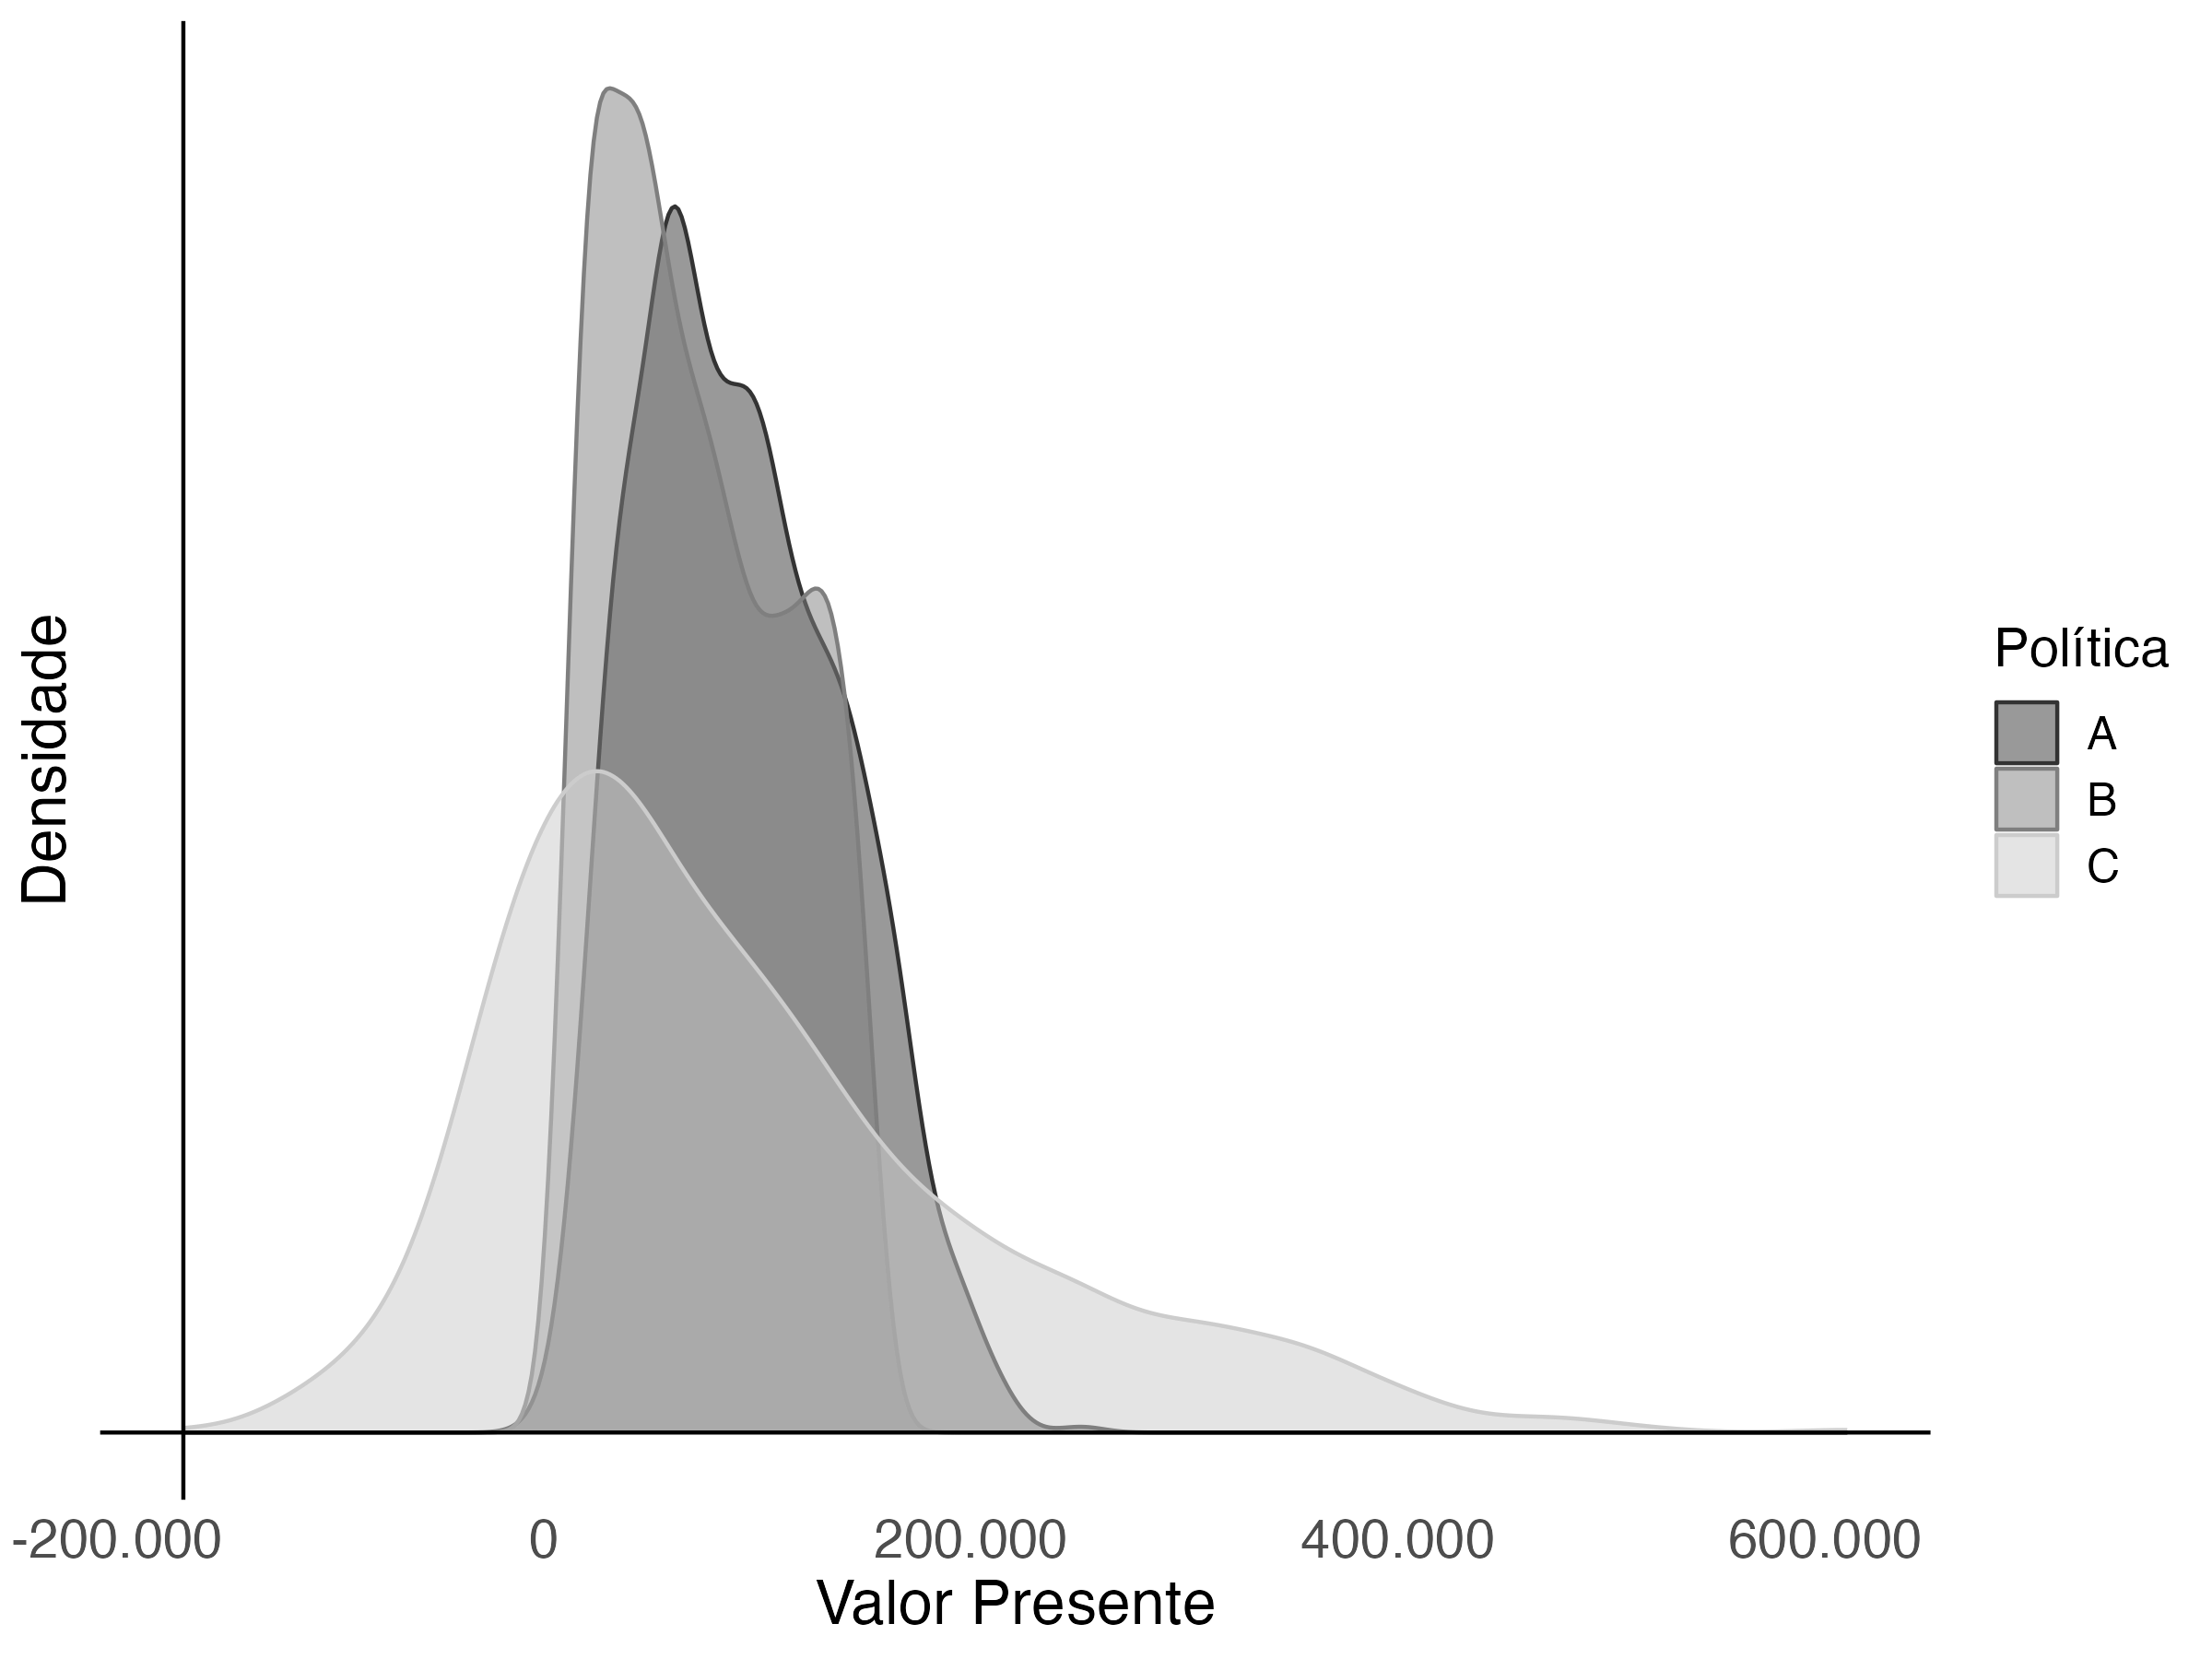
\includegraphics[scale=0.7]{Images/monte_carlo.png}
    \caption{Distribuição de Valores Presentes das Políticas A, B e C}
    \label{fig:montecarlodist}
\end{figure}

\newpage

\part*{Módulo 4}\label{mod:4}
\addcontentsline{toc}{part}{Módulo 4}

\section{Estudo de caso}

Neste módulo, exploram-se dois estudos de caso que examinam a eficácia e a viabilidade econômica de políticas educacionais que utilizam métodos de ensino diferentes e recursos complementares para promover o aprendizado. Cada caso ilustra os desafios e as metodologias necessárias para mensurar impactos, analisar custos e benefícios e estimar efeitos de longo prazo para indivíduos e para a sociedade.

O primeiro estudo de caso, apresentado na seção \ref{subsec:livros_ou_notebook}, avalia o impacto de um programa educacional em Honduras que substitui livros didáticos físicos por livros digitais acessados em notebooks. Esse programa inclui a oferta de dispositivos eletrônicos, treinamento e infraestrutura de internet, buscando melhorar a aprendizagem dos alunos e familiarizá-los com ferramentas digitais. A análise concentra-se tanto na eficácia do material digital em comparação aos livros físicos quanto no custo-benefício da implementação em grande escala.

Em seguida, o segundo estudo de caso analisa um programa educacional aplicado à pré-escola na cidade de Ypsilanti, Michigan, nos Estados Unidos. O programa Perry Preschool, implementado na década de 1960, visa aprimorar as habilidades cognitivas e socioemocionais das crianças por meio de atividades supervisionadas. A seção explica as metodologias empregadas para calcular a taxa de retorno do programa e para quantificar os benefícios e custos ao longo da vida dos participantes, especialmente em termos de ganhos educacionais e redução da criminalidade.

Por meio desses estudos de caso, este módulo busca apresentar abordagens práticas para conduzir uma Avaliação de Custo-Benefício (ACB) em contextos educacionais. A análise inclui considerações de impacto direto e indireto, externalidades, e avaliação do valor presente líquido dos benefícios e custos, facilitando uma compreensão robusta dos potenciais de cada intervenção.

\subsection{Livros ou Notebook?}
\label{subsec:livros_ou_notebook}

O estudo realizado por \textcite{bando2016books} avalia um programa de substituição de livros didáticos físicos por livros digitais em Honduras. Esse programa não apenas fornecia os livros didáticos digitais, mas também disponibilizava notebooks para os alunos, acesso à internet e treinamento para a utilização dos materiais digitais. O objetivo principal do estudo era analisar o impacto desse programa na aprendizagem dos alunos, comparando o desempenho acadêmico entre as escolas participantes do programa e as escolas que não participaram.

No entanto, além de avaliar a eficácia do ensino por meio de livros físicos ou digitais, é crucial considerar o custo-benefício de cada material didático para viabilizar o programa em larga escala. Embora o custo de um notebook geralmente seja mais alto, ele pode substituir vários livros didáticos. Portanto, é necessário comparar não apenas os benefícios de cada material didático, mas também seu custo.

A primeira etapa consiste em estimar o impacto do uso de livros físicos e digitais por meio de notebooks. Ao comparar o efeito de ambos os métodos, é comum na literatura calcular o efeito líquido entre a nova metodologia e a metodologia existente. Conforme discutido em seções anteriores, ao fazer a substituição, além do impacto dos livros digitais no aprendizado, também há o custo de oportunidade associado à interrupção do uso dos livros físicos e, consequentemente, à perda dos benefícios destes últimos. A diferença entre os efeitos nos fornecerá o impacto do uso de notebooks para aprendizado, menos o custo de oportunidade de não mais utilizar materiais físicos. Trataremos desse ponto na seção \ref{sub:ava_imp}.

No entanto, além do benefício líquido direto (que pode ser negativo ou zero) do uso dos notebooks, os autores argumentam que a literatura mostra uma externalidade positiva na utilização por crianças e adolescentes da tecnologia no ambiente escolar. As habilidades de alfabetização digital abrangem a capacidade de usar efetivamente as tecnologias digitais, navegar em plataformas online, acessar informações e utilizar ferramentas digitais para diversos fins. Essas habilidades são cada vez mais valiosas na era digital atual, pois são essenciais para o sucesso em muitas empreitadas educacionais, profissionais e pessoais.

A literatura sobre o tema também mostra que essas habilidades adquiridas acabam por elevar o potencial de ganhos futuros desses jovens quando eles adentrarem no mercado de trabalho o que ela chama de prêmio salarial da alfabetização digital (\textit{Digital literacy wage premium}). Ou seja, além do efeito direto, temos também o efeito de longo prazo no potencial salarial dos jovens que utilizam o ambiente digital para estudo. Na seção \ref{sub:ext_wage_premium} discutiremos como os autores estimaram esses efeitos.

Por fim, uma parte importante da avaliação de custo-benefício é a estimativa do custo marginal por aluno da utilização de ambas as metodologias de ensino, o que será abordado na seção \ref{sub:custo}.

\subsubsection{Avaliando o impacto do programa} \label{sub:ava_imp}

Para a avaliação, os autores em conjunto com o governo de Honduras selecionaram aleatoriamente 271 escolas de educação básica. Dentre essas, um grupo foi tratado, recebendo notebooks, infraestrutura de internet e treinamento para os alunos, enquanto outro grupo, o de controle, continuou a utilizar o material físico padrão sem receber nenhum computador ou infraestrutura tecnológica.

\vspace{5mm}

\begin{tcolorbox}[colback=gray!10,colframe=gray!50!black]

    \textbf{Grupo de Tratamento}: As escolas no grupo de tratamento receberam notebooks com conteúdo digital e acesso à Internet, substituindo os livros didáticos tradicionais para espanhol e matemática. Além de um treinamento para a utilização do material digital.
    
    \textbf{Grupo de Controle}: As escolas no grupo de controle continuaram a utilizar livros didáticos tradicionais para instrução sem receber notebooks.
\end{tcolorbox}

Os resultados foram avaliados dois anos após o início do programa. Para medir o efeito do programa na aprendizagem dos alunos, foram comparadas as notas entre os grupos de tratamento e controle para a terceira e sexta série do ensino fundamental. A Tabela \ref{tab:results} apresenta o impacto da substituição de livros didáticos por notebooks no desempenho dos alunos, com diferentes especificações de controle.\footnote{Nesta tabela, os resultados acadêmicos agregam as notas em matemática e espanhol, enquanto os resultados não acadêmicos, as notas em verbal e programação. Todos os resultados apresentados estão em desvio padrão.}

Para a terceira série, os resultados mostram que a substituição dos livros didáticos por notebooks teve um impacto negativo e estatisticamente significativo no desempenho dos alunos em testes acadêmicos de matemática e espanhol, quando comparado ao grupo que utilizou livros didáticos. No entanto, não houve diferenças significativas nos testes não acadêmicos de habilidades verbais e de programação. Para a 6ª série, os resultados indicam que a substituição dos livros didáticos por notebooks teve um impacto negativo e estatisticamente significativo no desempenho dos alunos em testes acadêmicos de matemática e espanhol. Novamente, não houve diferenças significativas nos testes não acadêmicos de habilidades verbais e de programação. 


\begin{table}[!htb] 
\centering
\footnotesize
\renewcommand{\arraystretch}{0.7} % Reduzir a altura das linhas da tabela
\setlength{\tabcolsep}{2pt} % Reduzir o espaçamento entre as colunas
\begin{adjustbox}{max width=0.95\textwidth,max totalheight=0.95\textheight,keepaspectratio,center}
\begin{tabular}{lcccccc}
\hline
 &  & & \multicolumn{4}{c}{\textbf{\begin{tabular}{c} Diferença das médias do grupo com notebooks menos \\ grupo com livros didáticos \end{tabular}}} \\

 \textbf{Variável} & \textbf{\begin{tabular}{ccc} Médias no \\ grupo com \\ livros didáticos \end{tabular}} & \textbf{\begin{tabular}{c} Sem \\ Controles \end{tabular}} & \textbf{\begin{tabular}{c} Controles \\ para área \\ rural e \\ status \\ fronteiriço \end{tabular}} & \textbf{\begin{tabular}{c} Controles \\ para \\ características \\ de alunos, \\ professores e \\ escolas \end{tabular}} & \textbf{\begin{tabular}{c} Diferença \\ em \\ Diferenças \end{tabular}} & \textbf{\begin{tabular}{c} P-valor \\ FWER  \end{tabular}} \\
\hline
 & \textbf{(1)} & \textbf{(2)} & \textbf{(3)} & \textbf{(4)} & \textbf{(5)} & \textbf{(6)} \\
\textbf{Painel A. 3º ano} &  &  &  &  &  \\
\hspace{2mm} Testes acadêmicos & 0.59 & -0.13** & -0.06 & -0.08** & -0.07* & 0.161 \\
& (0.80) & (0.07) & (0.06) & (0.04) & (0.04) & \\
\hspace{2mm} Matemática & 0.63 & -0.13* & -0.06 & -0.09 & -0.11** & 0.303 \\
& (0.92) & (0.08) & (0.07) & (0.06) & (0.06) & \\
\hspace{2mm} Espanhol & 0.59 & -0.14** & -0.06 & -0.06 & -0.04 & 0.303 \\
&(0.86) & (0.07) & (0.06) & (0.04) & (0.04) & \\
\hspace{2mm} Testes não acadêmicos & -0.00 & -0.05 & -0.03 & -0.02 & 0.05 & 0.938 \\
&(0.61) & (0.05) & (0.05) & (0.04) & (0.06) & \\
\hspace{2mm} Verbal & 0.14 & -0.07 & -0.07 & -0.01 & 0.09 & 0.938 \\
&(0.95) & (0.07) & (0.07) & (0.06) & (0.08) & \\
\hspace{2mm} Programação & -0.04 & -0.04 & -0.02 & -0.03 & -0.02 & 0.873 \\
&(0.66) & (0.05) & (0.05) & (0.05) & (0.09) & \\
\textbf{Painel B. 6º ano} &  &  &  &  &  \\
\hspace{2mm} Testes acadêmicos & 0.39 & -0.10 & -0.06 & -0.08** & -0.07 &  0.139 \\
& (0.79) & (0.06) & (0.06) & (0.04) & (0.04) \\
\hspace{2mm} Matemática & 0.56 & -0.13 & -0.10 & -0.14** & -0.10* & 0.139 \\
& (1.03)  & (0.09) & (0.09) & (0.06) & (0.06) \\
\hspace{2mm} Espanhol & 0.32 & -0.09 & -0.05 & -0.06 & -0.05 & 0.303 \\
& (0.84) & (0.06) & (0.06) & (0.04) & (0.04) \\
\hspace{2mm} Testes não acadêmicos & -0.12 & 0.01 & 0.03 & 0.06 & 0.10 & 0.532 \\
& (0.60) & (0.05) & (0.05) & (0.05) & (0.06) \\
\hspace{2mm} Verbal & -0.04 & 0.06 & 0.08 & 0.11** & 0.15* & 0.237 \\
& (0.82) & (0.07) & (0.07) & (0.06) & (0.08) \\
\hspace{2mm} Programação & -0.17 & -0.03 & -0.01 & 0.02 & 0.07 & 0.938 \\
& (0.71) & (0.06) & (0.06) & (0.06) & (0.08) \\
\hline
\multicolumn{7}{l}{Notas: Baseado em uma amostra de 9.600 alunos. Todas as estimativas de diferenças nas colunas (3) a (5) incluem} \\

\multicolumn{7}{l}{efeitos fixos de estratos. Os controles para a coluna (4) são todas as variáveis listadas na Tabela 2. Os valores de p} \\
\multicolumn{7}{l}{na coluna (6) são taxa de erro familiar estimada seguindo a metodologia descrita em Haushofer e Shapiro (2013).} \\
\multicolumn{7}{l}{Fonte: Tabela 4 \cite{bando2016books}.}
\end{tabular}
\end{adjustbox}
\caption{Impacto da substituição de livros didáticos por notebooks no desempenho dos alunos.} \label{tab:results}
\end{table}

Os resultados são apresentados com e sem controles para status rural e de fronteira, bem como para variáveis de alunos, professores e características da escola. A inclusão desses controles nas estimativas de diferenças destaca a importância de considerar esses fatores ao avaliar o impacto da substituição de livros didáticos por notebooks no desempenho dos alunos. Em resumo, os autores concluem que a substituição de livros didáticos por notebooks não teve um efeito positivo significativo no desempenho dos alunos, com resultados consistentes em diferentes séries e disciplinas. 

Ou seja, como estamos avaliando a diferença de impacto entre utilizar o material digital e o físico, a ausência de efeitos significantes sugere que ambas as abordagens tem o mesmo potencial de aprendizado nos alunos. Isso implica que em termos apenas de nível de aprendizado ambas as metodologias são equivalentes, i.e, independe de qual é usada.  

\subsubsection{Externalidade positiva: O Prêmio salarial da alfabetização digital} \label{sub:ext_wage_premium}

Como argumentado pelos autores, além do efeito direto no aprendizado, também há um efeito indireto através do Prêmio salarial da alfabetização digital. Isso ocorre porque adquirir habilidades digitais aumenta o potencial de salário futuro daqueles que são alfabetizados por meios digitais. Essa valorização acontece devido ao desenvolvimento de habilidades relevantes para o mercado de trabalho no futuro.

O artigo estimou o prêmio salarial da alfabetização digital de forma conservadora, assumindo um que este fosse de um por cento. Esse valor foi considerado baixo em comparação com as correlações relatadas em estudos anteriores, como \cite{krueger1993computers} e relatórios do \cite{world2016world}. Além disso, o artigo realizou uma análise de sensibilidade em relação a esse prêmio salarial, considerando diferentes cenários e taxas de desconto.


Para estimar o prêmio salarial da alfabetização digital, o artigo considerou a idade dos alunos no momento da avaliação e a média de anos de escolaridade para estimar o salário esperado no futuro dos participantes utilizando um modelo de regressão linear.

Entretanto, ainda é necessário levar em conta o desemprego geral no pais ($U$) e a participação no mercado de trabalho durante a vida dos jovens do programa ($P$). Para estimar o primeiro, eles utilizam a taxa de desemprego já o segundo, estimam com base nas características dos jovens, principalmente escolaridade. Esses dados foram utilizados para calcular o benefício esperado da alfabetização digital em cada período $t$ da vida profissional dos indivíduos usando a equação abaixo: 

\[
DLWP(t) = (1-U)P \left(\frac{{E[w | Esc]}}{\gamma^t}\right),
\]

\noindent onde \( DLWP(t) \) representa o Prêmio salarial da alfabetização digital (\textit{Digital literacy wage premium}) \(t\) períodos a partir de hoje. \( \text{{Esc}} \) é a média de anos de escolaridade no país, \( U \) é a taxa de desemprego, \( E[w | Esc] \) é o salário esperado de um aluno dado o nível de escolaridade média da população hondurenha, \( \gamma \) é a taxa de desconto intertemporal, definida como \( (1+r) \) onde \( r \) é a taxa de juros real da economia de Honduras, e \( P \) é a taxa de participação no mercado de trabalho em Honduras. Por fim, $(1-U)P$ calcula a proporção da população que está ativa no mercado de trabalho, isso é usado para estimar qual a probabilidade daquele aluno no futuro estar no mercado de trabalho formal.

O premio de risco será o valor presente líquido dos prêmios salariais líquidos ao longo da vida produtiva dos participantes:

\[DLWP = \sum_{t=t_0}^{t_0 + T} (1+0.01)^{t-t_0} \times DLWP(t)\]

\noindent \(t_0\) é a diferença da idade média de entrada no mercado de trabalho e a idade atual do estudante, e \(T\) é a quantidade média de anos no mercado de trabalho hondurenho. \((1+0.01)^t\) representa a taxa de crescimento do salário ao ano. Os autores argumentam que colocaram uma taxa média de 1\% que é muito menor que o realizado nos últimos anos em Honduras para serem conservadores.

Calculando o valor anual de DLWP para os parâmetros de honduras \cite{bando2016books} estimaram um prêmio salarial de aproximadamente U\$ 35,00 por aluno/ano. 

\subsubsection{Custo de cada metodologia} \label{sub:custo}

Os custos da metodologia digital foram calculados diretamente usando os custos efetivos durante a implementação do programa ou pela média de gasto do governo hondurenho.

O custo de provisão de notebook (-76 USD por aluno) foi calculado com base no custo de aquisição e distribuição dos notebooks para as escolas participantes do estudo. O custo de assistência técnica relacionada a notebooks (-5 USD por aluno) foi estimado considerando os custos de suporte técnico para garantir o funcionamento adequado dos notebooks nas escolas participantes durante o ano. Os custos de Internet e funcionamento dos notebooks (-9 USD por aluno) foram calculados levando em conta os gastos com conexão à Internet e despesas operacionais dos notebooks ao longo do período do estudo. O custo de treinamento do diretor para o uso da tecnologia (-5 USD por aluno) foi estimado com base nos custos associados à capacitação dos diretores das escolas para integrar efetivamente os notebooks no ambiente educacional médio que o governo hondurenho desembolsou durante os anos do estudo. O prêmio salarial de U\$35 dólares foi calculado como discutido na seção \ref{sub:ext_wage_premium}.

Já o custo do material didático é disponibilizado pelo governo hondurenho e é de U\$ 14 dólares por livro por aluno.

\subsubsection{Analise de Custo-Benefício}

Como ambas metodologias têm o efeito de aprendizado igual, para determinarmos entre as duas políticas qual seria mais eficiente, basta conseguirmos estimar o custo marginal de cada política. O custo marginal (por aluno) é de U\$ $14 \times$ Quantidade de livros para o material físico. Durante o experimento, 2 livros (linguagens e matemática) foram substituídos pelos materiais didáticos digitais, ou seja, um custo marginal por aluno de U\$ 28.

Já o benefício presente líquido\footnote{Já descontando a externalidade positiva do Prêmio Salarial por Alfabetização Digital.} por aluno de se trocar livros por notebooks é de - U\$ 63 que engloba tanto o custo da compra e manutenção dos laptops como custo de infraestrutura e treinamento. O resumo de cada custo está na tabela abaixo:

\begin{table}[h]
\centering
\begin{tabular}{l|r}
\hline
\textbf{Item de Custo} & \textbf{Laptops (USD)} \\
\hline
Fornecimento de Laptop & -76 \\
Assistência Técnica Relacionada a Laptop & -5 \\
Custos de Internet e Funcionamento do Laptop & -9 \\
Treinamento Principal para Uso da Tecnologia & -5 \\
\hline
\textbf{Custo Total} & \textbf{-95} \\
\hline
Prêmio Salarial por Alfabetização Digital & 35 \\
\hline
\textbf{Externalidade: Benefício Total} & \textbf{35} \\
\hline
\textbf{Custo Marginal Líquido} & \textbf{-63} \\
\hline
\multicolumn{2}{l}{Fonte: Elaboração própria} \\
\end{tabular}
\caption{Cálculo do Benefício Presente Líquido}
\end{table}

\textcite{bando2016books} argumentam, portanto, que trocar o material físico por notebooks não foi eficiente. Entretanto, como o custo marginal do material digital não aumenta com o número de materiais sendo sempre U\$ 63 diferentemente do material físico que custa U\$ 14 por material, Ao substituirmos 5 ou mais livros físicos o programa torna-se viável (custo de 5 livros = $5*14 = 70 < 63$ = custo do material digital).

Os autores deste artigo optaram por utilizar a métrica do benefício presente líquido para fazer a recomendação. Neste caso, em que não estamos comparando diferentes políticas, mas apenas verificando se uma determinada política aumenta o bem-estar da sociedade em relação ao \textit{status-quo}, a conclusão é indiferente à escolha da métrica utilizada.

Em síntese, o estudo avaliou o impacto da substituição de livros didáticos por notebooks em escolas de Honduras, analisando tanto os efeitos no aprendizado dos alunos quanto os custos associados à implementação da tecnologia digital. Os resultados indicam que, em termos de desempenho acadêmico, não houve ganhos significativos com a transição para notebooks, e em alguns casos, houve impactos negativos. No entanto, a digitalização do ensino pode gerar externalidades positivas de longo prazo, como o prêmio salarial da alfabetização digital, que reflete o aumento no potencial de ganhos futuros dos alunos.

A análise de custo-benefício mostrou que, embora a substituição de dois livros por notebooks não seja economicamente vantajosa, o modelo torna-se viável se ao menos cinco livros forem substituídos. Assim, a adoção da tecnologia como ferramenta educacional deve considerar não apenas seu impacto imediato na aprendizagem, mas também seus custos e benefícios de longo prazo para garantir uma implementação eficiente e sustentável.

\subsection{Taxa de retorno do Programa Perry Preschool}

O programa estudado foi feito na pre-escola Perry na cidade Ypsilanti no Michigan durante o começo dos anos 60 e consistia em aulas orientadas das crianças participantes do programa complementada por visitas domiciliais de professores.  

O currículo do programa basea-se em atividades para auxiliar e incentivar o aprendizado cognitivo e socio-emocional das crianças por meio de atividades orientadas e supervisionadas por professores treinados. As crianças eram encorajadas a sempre a fazer as tarefas e atividades propostas e a refletir sobre suas ações depois das atividades e durante todo o processo os professores foram orientados a incentivarem as crianças a manterem-se engajadas nas atividade. 

O programa enfatizava em vez de um currículo focado em lições passivas, um ensino mais reflexivo e com questionamentos mais amplos para os alunos. Durante as atividades, as crianças eram colocadas em situações para que tomassem suas próprias decisões e a resolver por si só problemas colocados a elas. Além disso, eram questionadas depois das atividades com frases mais abertas como: "O que houve?, Como você fez isso? Você poderia me mostrar como? Você conseguiria ajudar outras crianças?" para incentivar a reflexão tanto cognitiva quanto socio-emocional por parte do aluno \cite{heckman2010rate}. 

Após o tratamento, os participantes foram acompanhados ao longo de 40 anos e diversas informações foram coletadas por meio de pesquisas anuais. Alguns dos temas dessas pesquisa eram, por exemplo, educação, emprego, salário e criminalidade. Entretanto, para avaliar o beneficio do programa, temos inúmeros problemas. O primeiro é como agregar os efeitos em áreas tão diferentes como o salario médio, anos de educação e a probabilidade de se cometer crime e etc. Segundo, o programa tem como efeito a geração de externalidades para toda sociedade: ao diminuir a probabilidade de crimes você acaba diminuindo os custos com detenções, a criminalidade do país e etc. E, por fim, um terceiro problema é como comparar os benefícios, que por vezes são não monetários, com os custos do programa. 

Neste sentido, os autores construíram uma taxa de retorno do programa que tem como objetivo estimar e quantificar na mesma unidade de medida os custos e benefícios tanto privados quanto sociais do programa. Vamos tratar cada uma delas ao longo desse estudo de caso e como os autores fizeram para construir essa taxa de retorno que é uma medida do custo benefício do programa como um todo. Como estamos mais interessados na parte da construção do custo e do benefício, passaremos rapidamente pela identificação e estimação dos efeitos e focaremos mais em como esses efeitos são agregados e quantificados na mesma unidade de medida. 

\subsubsection{A avaliação do impacto do Programa} \label{sec:avaliacao_heckman}

Durante a implementação do programa, os participantes foram aleatorizados entre um grupo de tratado e controle. Assim, os efeitos médios foram avaliados como a diferença em média do grupo de tratamento contra a diferença em média do grupo de tratado. Isso é possível pois, a aleatorização garante a exogeneidade do tratamento. 

\textcite{heckman2010rate} argumentam que houveram problemas na aleatorização como um número não desprezível de \textit{always takers},\footnote{Participantes que independentemente de terem ou não sido selecionados de forma aleatória para participar do programa acabam por participar dele.} problemas na elegibilidade ao programa, entre outros. Não vamos entrar no mérito de como os autores resolveram cada um desses problemas, pois não é o foco dessa publicação. 

Por fim, muitos dos benefícios e custos do programa avaliados não estavam na mesma unidade de medida (em unidades monetárias), portanto, parte importante do processo foi fazer essa mudança. Por exemplo, um dos benefícios avaliados é a diminuição da probabilidade do jovem e adulto cometer crimes no futuro. Para a avaliação de custo-benefício, os autores tiveram que quantificar benefícios não monetários, como essa probabilidade, em unidades monetárias.

Abaixo resumimos cada um dos benefícios e custos avaliados no programa:

\textit{Benefícios}

\begin{itemize}
    \item \textbf{Educação}. O benefício mais direto do programa é avaliado em dois principais resultados: a frequência e as notas durante não só o período do programa mas ao longo da vida escolar da pessoa.

    \item \textbf{Emprego e renda}. Benefícios tanto privado quanto social são as rendas e a presença no mercado de trabalho. Para o individuo uma maior renda gera um bem-estar geral maior e para a sociedade isso impacta na renda média de todos via multiplicador. 
    
    \item \textbf{Crime}. Estudos na área da criminalidade demonstram que tanto a educação mais formal (escolar ou acadêmica) quanto a educação na forma de socialização garantem melhores oportunidades para as pessoas na vida adulta. Com mais oportunidades, a incidência de crimes tende a diminuir. Entretanto, esse cálculo não é trivial, uma vez que demanda estimar atividade criminal e custos sociais do crime para grupos de controle e tratamento.\footnote{\textit{"Estimating the impact of the program on crime requires estimating the true level of criminal activity at each age and obtaining reasonable estimates of the social cost of each crime."} \cite{heckman2010rate}}

    Para isso eles dividem o custo do crime em 3 principais: \textit{custo da vítima}, ou seja, o custo tanto monetário quanto psicológico da vitima; \textit{custo do policiamento} que representa os custos de pessoal, administrativo e etc. da força policial. Por fim, \textit{custo de encarceramento} que representa o custo para o estado das punições à cada indivíduo.

    \item Impostos

    Outro benefício é o aumento do imposto que o estado coleta devido à uma renda possivelmente maior e uma presença maior no mercado de trabalho formal das pessoas que foram tratadas. 
    
\end{itemize}

\textit{Custos}

\begin{itemize}
    \item \textbf{Educação}. A educação, entretanto, não tem só benefícios. Há custos como salário dos professores, infraestrutura, auxílios de permanência e materiais didáticos, por exemplo. Os autores calcularam também o chamado \textit{k-12 cost}, que representa o custo durante os 12 anos de educação básica americana por aluno. 
    
    No caso do Estados Unidos, temos, além desse custo, um tipo especial de educação como o Desenvolvimento Educacional Geral (GED, na sigla em inglês). Esse tipo de educação é mais cara que a educação padrão e o programa aumenta a probabilidade, principalmente das meninas tratadas, de participação desse tipo de educação no futuro. 

    Os autores também estimam o custo da educação universitária. Eles dividem em dois tipos de custos: o primeiro\footnote{\textit{College, age < 27} } que representa os custos de educação universitária padrão antes dos 27 anos e o segundo\footnote{\textit{Education, age > 27}} que representa custos de educação superior posterior à 27 anos ao qual os dados eram mais escassos em relação a que tipo de cursos e qual o financiamento do mesmo. Em função disso, esse segundo grupo de custos foi estimado de maneira mais superficial pelos autores.
    
    Nos Estados Unidos há também cursos de treinamento vocacional opcionais ao longo da vida escolar dos alunos. Os custos por alunos também foram levantados pelos autores.

    \item \textbf{Custo-benefício dos programas sociais}. Boa parte dos participantes do programa, ao longo da sua vida, receberam auxílios financeiros ou não. Esses auxílios compreendem desde de auxílios para alimentação como moradia, educação e etc. Esses auxílios transferem renda de parte da população  via impostos para outra via essas transferências. \cite{heckman2010rate} estimou o efeito líquido total desses programas. 
    
\end{itemize}

\subsubsection{Estimação dos custos e dos benefícios do Programa}

{\large \textbf{Benefícios e custos em unidades monetárias}}

\textbf{Emprego e Renda}, \textbf{impostos} e os \textbf{custos da educação} já estão avaliados na unidade de medida correta. Todos são medidos em valores monetários. O único ajuste que se fez necessário para os autores foi extrapolar a renda dos participantes após quarenta anos de idade. Eles tinham apenas a renda até 40 anos via as pequisas periódicas feitas. Sendo assim, eles usaram um modelo de renda ao longo da vida para estimar os efeitos para mais de 40 anos de idade. 

{\large \textbf{Crimes}}

Para atribuir valores monetários aos crimes, os pesquisadores adotaram uma abordagem cuidadosa e detalhada. Eles consideraram não apenas o impacto direto do crime em termos de custos de justiça criminal e danos materiais, mas também os custos intangíveis, como o sofrimento das vítimas e suas famílias. Além disso, foi levado em conta o efeito cascata dos crimes, ou seja, como um crime pode levar a outros crimes e custos adicionais para a sociedade.

Para crimes como assassinato e crimes relacionados a drogas e direção, que foram considerados como tendo vítimas diretas, os pesquisadores avaliaram os custos associados aos processos judiciais, tratamento médico, perda de produtividade e impacto emocional nas vítimas e suas famílias. Esses custos foram quantificados com base em dados de custos médicos, salários perdidos e estudos sobre o impacto psicológico de tais crimes.

Por outro lado, para crimes considerados "sem vítimas", como dirigir sob efeito de álcool e crimes relacionados a drogas, os pesquisadores adotaram uma abordagem mais complexa. Eles consideraram os custos indiretos desses crimes, como o impacto na segurança pública, custos de aplicação da lei, custos de tratamento de dependência química e os efeitos indiretos na economia local.

Além disso, os pesquisadores também levaram em conta o efeito cascata dos crimes, ou seja, como um crime pode levar a outros crimes e custos adicionais para a sociedade utilizando os resultados da literatura de crimes existentes.

Por fim, para estimar o impacto do programa sobre a criminalidade, é necessário determinar o nível real de atividade criminosa em cada idade e obter estimativas razoáveis do custo social de cada crime. Para um crime do tipo $c$ no tempo $t$, o custo social total desse crime, $V^t_c$, pode ser calculado como o produto do custo social por unidade de crime, $C^t_c$, e a incidência $I^t_c$:

\[ V^t_c = C^t_c \times I^t_c \]

$I^t_c$ que é a incidência real de crimes para cada grupo não é observada, entretanto, o registro de prisões de cada sujeito na idade $t$ para o crime $c$, $A^t_c$ é conhecida por meio das pesquisas anuais. Buscando a relação incidência-prisão $I^t_c/A^t_c$ de outras fontes de dados, os autores estimaram $V^t_c$ multiplicando os três termos:

\[ V^t_c = C^t_c \times \left(\frac{I^t_c}{A^t_c}\right) \times A^t_c \]

Para obter a relação incidência-prisão $I^t_c/A^t_c$ para cada tipo de crime $c$ no tempo $t$, eles utilizaram dois conjuntos de dados americanos sobre crimes: o \textit{Uniform Crime Report} (UCR) e a \textit{National Crime Victimization Survey} (NCVS). 

As tipologias de crimes derivadas do UCR e do NCVS "não são estritamente comparáveis" como argumentado por \cite{heckman2010rate}. Para superar esse problema, eles desenvolveram uma categorização unificada de crimes entre os conjuntos de dados NCVS, UCR e Perry para crimes graves e contravenções. Para verificar a sensibilidade dos resultados à escolha de uma categorização específica de crimes, eles usaram dois conjuntos de relações incidência-prisão: para o primeiro conjunto, assumiram que cada tipo de crime tem uma relação incidência-prisão diferente, denotadas como \textit{``separated"}. Para o segundo conjunto, são usadas duas categorias amplas, crime violento versus crime contra a propriedade, denotadas como \textit{``Property vs. violent"}.

{\large \textbf{Efeito total ao longo da vida}}

A Tabela 3, resume cada um dos custos e benefícios tratados acima tanto para homens como para mulheres. A coluna \textit{separate} representa a estimação dividindo entre os tipos de classificação de crimes. Todos os valores foram trazidos a valor presente em dólares de 2006. O \textit{Lifetime effect} representa o efeito total do tratamento, isto é, custo/benefício total dos tratados menos custo/benefício total dos controles. 

\begin{figure}[H]
    \centering
    \includegraphics[width=1\textwidth]{Murilo/table3_heck.png}
    {\small Tabela 3 pagina 119 de \cite{heckman2010rate}}
\end{figure}


\subsubsection{Imputação e extrapolação}

Os autores tiveram dois outros problemas para lidar: as ausências de informação em algum momento ao longo do tempo dos participantes seja porque eles não responderam à pesquisa ou porque alguma informação específica não estava disponível por algum motivo e a falta de dados após os 40 anos de idade dos participantes. 

Para lidar com o primeiro, os autores usaram diversos métodos de imputação das informações faltantes, para garantir que os resultados serão consistentes aos diferentes métodos: \textit{Piecewise linear interpolation}, \textit{Cross-sectional regression}, \textit{Kernel matching} e o método proposto por \cite{hause1980fine}. 

Para a extrapolação, eles também usaram diferentes metodologias para garantir que os resultados eram robustos a todas elas. A primeira foi retirar da pesquisa \textit{Current Population Survey (CPS)} os ganhos médios esperados via média móvel de três anos com base na educação, gênero e raça chamada apenas de \textbf{CPS}. A segunda é utilizar os dados disponíveis em \textit{Panel Study of Income Dynamics (PSID)} pesquisa na qual se determina os ganhos para cada perfil de indivíduo e, posteriormente, extrapolar os ganhos via um modelo de efeitos aleatórios usando variáveis indicadoras de idade, educação além de uma constante e os ganhos passados. A esse método os autores se referiram por \textbf{PSID} Por fim, eles estimam os ganhos esperados futuros usando a metodologia proposta por \cite{hause1980fine}.

\subsubsection{Taxa Interna de Retorno do Programa (IRR)}

Como a avaliação do custo e benefício do programa lida com fluxos ao longo do tempo apenas colocar na mesma unidade de medida, como dinheiro, não é suficiente. Então, a literatura comumente utiliza a taxa interna de retorno. Isso facilita a comparação de diferentes tipos de projetos com tempos de execução e ganhos variados. 

A Tabela 5 resume as IRRs, em porcentagem, para diferentes tipos de imputação e extrapolação. Os autores também dividiram entre o custo-benefício privado (\textit{To individual)} e o social (\textit{To Society}), este último abarcando o custo privado e as externalidades positivas e negativas do programa discutidos na seção \ref{sec:avaliacao_heckman}.

Para estimar o custo dos crimes eles utilizaram três formas. A primeira e a segunda, chamada de \textit{Separate high} e \textit{Separate low}, estimam o custo de cada crime separadamente dando um valor de assassinato alto (\textit{Separate high}) de 4.3 milhões de dólares e outro mais conservador,\textit{Separate low}, de 13 mil dolares. \footnote{O custo High considera o custo total para a sociedade com o assasinato calculando o quanto era esperado de salário durante a vida do assassinado, em média. Enquanto o custo low refere-se ao custo apenas privado do assasinato sendo uma das mais conservadoras estimativas da literaturas do tema.}

Por fim, eles estimam o custo dos crimes agrupando, chamado de \textit{Property vs violent}, em apenas duas categorias de crimes: contra propriedade e crimes violentos.  Nessa categoria, em vez de estimarem todos a probabilidade de cada crime individualmente eles estimam apenas a probabilidade de crimes contra a propriedade (que não resultam em morte) e contra a vida (que resultam em morte). Para os crimes contra a vida eles utilizam o custo social mais baixo, ou seja, 13 mil dolares por assasinato.

\begin{figure}[!htp]
    \centering
    \includegraphics[width=1\textwidth]{Murilo/tab5.png}
    {\small Tabela 5 pagina 123 de \cite{heckman2010rate}}
\end{figure}

Com alguma variabilidade, a taxa de retorno do programa é sempre positiva variando de 5\% à 11\% sendo significativamente diferente de zero. Os desvios padrões foram estimados combinando re-sample com bootstrap. \cite{heckman2010rate} argumenta também que apesar de sua análise estimar taxas de retornos menores que a literatura existente até então ela ainda assim é positiva.

Há um problema ao se utilizar a taxa interna de retorno para avaliar o efeito de programas com grupo de tratado e controle. A IRR é solução de um polinômio que denota os fluxos ao longo do tempo da diferença entre os beneficio/custo do grupo de controle e do grupo de tratamento. Entretanto, possivelmente, podemos ter múltiplas raízes, ou até mesmo raízes complexas como solução desse polinômio. O que geraria um problema de qual das raízes é a taxa interna? A menor, a maior? Isso gera uma possibilidade de escolha arbitrária para o pesquisador. E, com raizes complexas, a dificuldade surge em como interpretar tal raiz. 

\cite{heckman2010rate} argumenta, entretanto, que em todas as análises apenas uma raiz real foi solução. Além disso, eles também calcularam o \textit{beneficit-to-cost ratio} e as conclusões se mantiveram. 


\newpage
\printbibliography
\end{document}